\documentclass[12pt,reqno]{amsart}

\usepackage{graphicx}
% \usepackage{mdframed}
\usepackage{amssymb}
\usepackage{amsthm}
\usepackage{mathrsfs}
\setlength{\parskip}{0.5\baselineskip}%
\setlength{\parindent}{20pt}
\renewcommand{\qedsymbol}{$\blacksquare$}

% theorem style changed
\theoremstyle{plain}
\newtheorem*{thm*}{Theorem}
%% this allows for theorems which are not automatically numbered
\newtheorem{thm}{Theorem}
\newtheorem{lem}{Lemma}
\newtheorem{cor}{Corollary}
\newtheorem{prop}{Proposition}

% theorem style changed
\theoremstyle{definition}
\newtheorem{defn}{Definition}
\newtheorem{exer}{Exercise}
\newtheorem{eg}{Example}
\newtheorem{rem}{Remark}
\newtheorem*{sol*}{Solution}


\newcommand{\bb}[1]{\mathbb{#1}}
\newcommand{\cal}[1]{\mathcal{#1}}
\usepackage{lineno}

%% The above lines are for formatting.  In general, you will not want to change these.


\title{General Topology}
\author{Devansh Tripathi}

\begin{document}

\begin{abstract}
    We shall learn some general topology. Rest of the abstract is left as an exercise to the reader.
\end{abstract}
\maketitle
\newpage
\begin{defn}
    Induced metric: A metric which is derived from a norm. A normed space is a special metric space whose metric is derived from a norm.
\end{defn}
\begin{eg}
    $\mathscr{C}[a,b]$: Set of all bounded continuous real function on a closed interval form the normed space with norm defined as $$ \|f\| = \int_a^b |f(x)|~dx \hspace{0.35cm}\text{or,} \hspace{0.5cm} \|f\| = \sup{|f(x)|}$$ and the induced metric is $$ \|f - g \| = \int_a^b |f(x) - g(x)| ~ dx \hspace{0.35cm} \text{or,} \hspace{0.5cm} \|f - g\| = \sup{|f(x) - g(x)|} $$
\end{eg}
\begin{defn}
    Distance of a point $x$ from a set $A$: $$ d(x, A) = \inf\{d(x,a) \mid \forall a \in A \} $$
    Diameter of the set: $$ d(A) = \sup \{d(a_1, a_2) \mid \forall a_1, a_2 \in A\} $$
\end{defn}
\begin{defn}
    Bounded mapping: A mapping $f$ of a non-empty set into a metric space is said to be bounded if its range is bounded i.e. $\exists M \in \mathbb{R} \text{ such that } |f(x)| \leq M $ 
\end{defn}
\begin{eg}
    A pseudo metric which is not a metric
    $$ f,g \in \mathbb{R}^2 \text{ and } d(f,g):= \text{difference between their $x$ coordinates} $$    
\end{eg}
\begin{defn}
    Interval: A set $A \subset \mathbb{R}$ is an interval if $$ \forall x, y \in A \text{ and } \forall t \in \mathbb{R} \colon x \leq t \leq y \implies t \in A $$ 
\end{defn}
\begin{thm}
    Union of intervals with non empty intersection is an interval.    
\end{thm}
\begin{proof}
    Let $\{I_i\}$ be the set of interval and $a \in \cap_i I_i$.\\
    Proof Idea: Take any two points in the union and show that they contains every point in between them (take general point and show that it will belong to the union).\\
    Let $x,y \in \cup_i I_i$ and let $t \in \mathbb{R} \colon x \leq t \leq y $ then there are following possiblities:\\
    $t < a$, \\$ t = a$ or, \\ $t > a$.\\ All are trivial to show that they lie in union.
\end{proof}
\section{Topological Spaces}
\begin{defn}
    Topology: A topology on a set $X$ is a collection $\mathcal T$ of subsets of $X$ having the following properties:
\begin{itemize}
    \item $\phi$ and $X$ are in $\mathcal T$.
    \item The union of the elements of any subcollection of $\mathcal T$ is in $\mathcal T$.
    \item The intersection of the elements of any finite subcollection of $\mathcal T$ is in $\mathcal T$.
\end{itemize}
\end{defn}
A set $X$ with topology $\mathcal T$ is called an topological space ($X,\mathcal T$).
\begin{defn}
    Open set of $X$: For the topological space $(X, \mathcal T)$, a subset $U$ of $X$ is an open set of $X$ if $U$ belongs to the collection $\mathcal T$.
\end{defn}
\begin{eg}
    Discrete Topology: If $X$ is any set then collection of all subsets of $X$ is a topology on $X$, called {\bf discrete topology.}
\end{eg}
\begin{eg}
    Indiscrete or trivial topology: The topology consisting of only $\phi$ and the whole set $X$ is called {\bf trivial topology.}
\end{eg}
\begin{eg}
    Finite complement topology: Let $X$ be a set and $\mathcal{T}$ be the collection of all subset $U$ of $X$ such that $X - U$ is either finite or $X$. Then $\mathcal{T}$ is called {\bf finite complement topology}. (This topology is consists of subset of $X$ whose complement is either finite or $X$.)
\end{eg}
\begin{proof}
    Let $\{U_{i}\}$ be the indexed family of subsets of $X$ belongs to $\mathcal{T}$. $\phi$ and $X$ are obviously there. Assume each $\bigcup\limits_i U_i$ is non-empty (trivial for empty case): 
    $$X - \bigcup\limits_i U_i = \bigcap\limits_i(X - U_i)$$
    Since each $U_i$ is in $\mathcal{T}$, $X - U_i$ is finite. and $\bigcap\liminf_i X - U_i$ is contained in every $X - U_i$ hence it is finite.\\ \\
    To show $\bigcap\limits_i^n U_i$ is in $\mathcal{T}$, 
    $$ X - \bigcap\limits_i^n U_i = \bigcup\limits_i^n (X - U_i) $$
    Rhs is finite union of finite sets hence it is finite.
\end{proof}
\begin{eg}
    Let $X$ be set and $\mathcal{T}_c$ be the collection of all subsets $U$ of $X$ such that $U^c$ is either countable or all of $X$. Then $\mathcal{T}_c$ is a topology of $X$. 
\end{eg}
\begin{proof}
    $\phi$ and $X$ are trivial inside $\mathcal{T}_c$. Let $U_i$ be the indexed family of subsets of $X$. Assume $\bigcup\limits_i U_i$ is non-empty (trivial for empty case). To show that $\bigcup\limits_i U_i$ is in $\mathcal{T}_c$
    $$ X - \bigcup\limits_i U_i = \bigcap\limits_i (X - U_i)$$
    Since, $X - U_i$ is countable for each $i$ and $\bigcap\limits_i (X - U_i)$ is in $U_i$ for each $i$. Hence, $\bigcap\limits_i (X - U_i)$ is countable. \\
    To show that $\bigcap\limits_i U_i$ is in $\mathcal{T}_c$, use the same argument as last example and the fact that finite union of countable sets is countable.
\end{proof}
\begin{defn}
    Finer or strictly finer topology: For a set $X$, if $\mathcal{T}$ and $\mathcal{T}'$ are two topologies on $X$ such that $\mathcal{T} \subset \mathcal{T}'$ then we say $\mathcal{T}'$ is {\bf finer} than $\mathcal{T}$ and if $\mathcal{T}'$ properly contains $\mathcal{T}$ then we say it's {\bf strictly finer}. Then $\mathcal{T}$ is called {\bf coarser} than $\mathcal{T}'$ or, {\bf strictly coarser} if it is contained in $\mathcal{T}'$ properly.
\end{defn}
\begin{defn}
    Comparable: We say $\mathcal{T}$ is comparable with $\mathcal{T}'$ if either $\mathcal{T} \subset \mathcal{T}'$ or $\mathcal{T}' \subset \mathcal{T}$.
\end{defn}
\section{Basis for a Topology}
\begin{defn}
    If $X$ is a set, a {\bf basis} for a topology on $X$ is a collection $\mathcal{B}$ of subsets of $X$ (called basis elements) such that
    \begin{itemize}
        \item For each $x \in X$, there is atleast one basis element $B \in \mathcal{B}$ such that $x \in B$.
        \item If $x$ belongs to the intersection of two basis elements $B_1$ and $B_2$, then there is $B_3 \in \mathcal{B}$ such that $x \in B_3 \subset B_1 \cap B_2$. 
    \end{itemize}
\end{defn}
We define a topology $\mathcal{T}$ generated by $\mathcal{B}$ as: A subset $U$ of $X$ is said to be open in $X$ (e.g. an element of topology on $X$) if for all $x \in U$, there is a basis element $B \in \mathcal{B}$ such that $x \in B \subset U$.

\begin{rem}
    Each element of the basis is an element of the topology. 
\end{rem}
\begin{eg}
    If $X$ is any set then the collection of all one element subsets of $X$ is a basis for the discrete topology on $X$.(Power set of $X$). 
\end{eg}
\begin{proof}
    Trivial to see. (Caution: Do not take element of the topology on $X$. For basis, condition is on the elements of the set $X$ hence take element of $X$ and then check basis conditions.)
\end{proof}
\begin{lem}
    The collection $\mathcal{T}$ generated by the basis $\mathcal{B}$ is a topology.
\end{lem}
\begin{proof}
    Let the collection $\mathcal{T} = \{U_i\}_{i \in I}$. Condition for the set $U_i$ to belong to the collection is that for each $x \in U_i$ there exists an element $B \in \mathcal{B}$ and $x \in B \subset U_i$.
    \paragraph{\bf Membership of $\phi$ and $X$:}
    For $\phi$, it is vacuously true (true due to non-availability of elements in the set). For $X$, for each $x \in X$, there exists $B \in \mathcal{B}$ (by definition of basis) such that $x \in B$ and $B \subset X$.
    \paragraph{\bf Closure under arbitray union of elements.} Now, assume that $\{U_i\}_{i \in I}$ is the indexed family of subsets of $X$ which are elements of $\mathcal{T}$. We need to show that $\bigcup\limits_{i \in I} U_i \in \mathcal{T}$. For each $x \in \bigcup\limits_{i} U_i \implies x \in U_i$ for some $i$ and $U_i \in \mathcal{T} \implies \exists B \in \mathcal{B} \text{ such that } x \in B \subset U_i$. This completes the argument.
    \paragraph{\bf Closure under finite intersection.} We need to show that $\bigcap\limits_{i = 0}^{n} U_i \subset \mathcal{T}$. For each $x \in \bigcap\limits_{i = 0}^{n} U_i$
    $$ x \in U_i ~~\forall i \implies \exists B_i \in \mathcal{B} ~~\forall i \in \{0,1,\dots n\}$$
    Since, $x \in \bigcap\limits_{i = 0}^{n} B_i$ and $B_i~'s$ are basis elements hence by definition of basis, $\exists B' \in \mathcal{B}$ such that $x \in B' \subset \bigcap\limits_{i = 0}^{n} B_i$. Hence, $\bigcap\limits_{i = 0}^{n} U_i \subset \mathcal{T}$.
\end{proof}
\begin{lem}
    Let $X$ be a set; $\mathcal{B}$ is the set of all basis elements of the topology $\mathcal{T}$ on set $X$. Then $\mathcal{T}$ equals the collection of all unions of elements of $\mathcal{B}$.
\end{lem}
\begin{proof}
    Since each element $B$ of basis is in $\mathcal{T}$ and hence their union. For other way around, let $U \in \mathcal{T}$, then for each $x \in U~~\exists B_x \in \mathcal{B} \subset U$ hence, $ U = \bigcup\limits_{x \in U} B_x$. Therefore, each $U \in X$ is union of basis elements.
\end{proof}
\begin{rem}
    Above lemma states that every set $U$ in $X$ can be expressed as union of basis elements of the topology, however this is {\bf not unique.}
\end{rem}
\begin{lem}
    Let $X$ be an topological space. Suppose that $\mathcal{C}$ is a collection of open sets of $X$ such that for each open set $U$ of $X$ and each $x \in U$, there is an element $C$ of $\mathcal{C}$ such that $x \in C \subset \mathcal{C}$. Then $\mathcal{C}$ is a basis of the topology of $X$.
\end{lem}
\begin{proof}
    First we will prove that $\mathcal{C}$ is the basis of the topology on $X$.
    \paragraph{\bf First condition of basis:} Since $X$ is a open set of itself hence hypothesis, by for each $x \in X$ there exists $C \in \mathcal{C}$ such that $x \in C \subset \mathcal{C}$.
    \paragraph{\bf Second condition of basis:} Let $x \in C_1 \cap C_2$ for some open sets $C_1, C_2 \in \mathcal{C}$. Since $C_1, C_2$ are open in $X$ then so is $C_1 \cap C_2$ hence by hypothesis for each $x \in C_1 \cap C_2$ there exists $C_3 \in \mathcal{C}$ such that $x \in C_3 \subset C_1 \cap C_2$.
    \paragraph{\bf Topology generated by $\mathcal{C}$ equals topology of $X$.} Let $\mathcal{T}_c$ be the topology generated by $\mathcal{C}$ and $\mathcal{T}$ be a topology on $X$. Let $U \in \mathcal{T}$. For each $x \in U$, by hypothesis, there exists $C_x \in \mathcal{C}$ such that $x \in C_x \subset U$ hence $U = \bigcup\limits_{x \in U} C_x$(union of elements of $\mathcal{C}) \implies \mathcal{T} \subset \mathcal{T}_c$.\\
    Let $V \in \mathcal{T}_c \implies V = \bigcup\limits_{i \in I} C_i$ for each $C_i \in \mathcal{C}$ (by previous lemma). Since each $C_i$ are open in $X$ hence $C_i \in \mathcal{T}$ and $\mathcal{T}$ is a topology (their union will belong to $\mathcal{T}$). Hence, $V \in \mathcal{T} \implies \mathcal{T}_c \subset \mathcal{T}$. Therefore, $\mathcal{T}_c = \mathcal{T}$.
\end{proof}
\begin{lem}
    Let $\mathcal{B}$ and $\mathcal{B}'$ be bases for the topologies $\mathcal{T}$ and $\mathcal{T}'$, respectively, on $X$. TFAE
    \begin{enumerate}
        \item $\mathcal{T}'$ is finer than $\mathcal{T}.$
        \item For each $x \in X$ and each basis element $B \in \mathcal{B}$ containing $x$, there is a basis element $B' \in \mathcal{B}'$ such that $x \in B' \subset B$.
    \end{enumerate}
\end{lem}
\begin{proof}
    $(1) \implies (2)$ (Idea is: Since $\mathcal{T} \subset \mathcal{T}'$, every set of $\mathcal{T}$ is a set in $\mathcal{T}'$. Hence, $B \in \mathcal{T}$ can be written in terms of basis of $\mathcal{T}'$)
    \par \noindent We assume that $\mathcal{T} \subset \mathcal{T}'.$ For all $x \in X$ there exists $B \in \mathcal{B}$ such that $x \in B \subset \mathcal{T}$. And $\mathcal{T} \subset \mathcal{T}' \implies B \subset \mathcal{T}'$. Therefore, there exists a $B' \in \mathcal{B}'$ such that $ \forall x \in B, x \in B' \subset B$.
    \paragraph{$(2) \implies (1)$} Assume $(2)$ and let $U \in \mathcal{T}$. We need to show that $U \in \mathcal{T}'$. For each $x \in U$ there exists $B \in \mathcal{B}$ such that $x \in B \subset U$. From condition $(2)$, there exists a $B' \in \mathcal{B}'$ such that $x \in B' \subset B \subset U \implies B' \subset U$. Therefore by definition of basis, $U \in \mathcal{T}' \implies \mathcal{T} \subset \mathcal{T}'$.
\end{proof}
\begin{defn}[Standard Topology on $\mathbb{R}$]
    If $\mathcal{B}$ is the collection of all open intervals in the real line
    $$ (a,b) = \{x \mid a < x < b\},$$
    the topology generated by $\mathcal{B}$ is called the {\bf standard topology} on the real line.
\end{defn}
\begin{defn}[Lower limit topology on $\mathbb{R}$]
    If $\mathcal{B}'$ is the collection of all half-open interval of the form 
    $$ [a,b) = \{x \mid a \leq x < b\},$$
    where $a < b$, the topology generated by $\mathcal{B}'$ is called the {\bf lower limit topology} on $\mathbb{R}$. $\mathbb{R}$ with this topology is denoted as $\mathbb{R}_l$.
\end{defn}
\begin{defn}[$K$-topology on $\mathbb{R}$]
    Let $K$ denote the set of all number of the form $1/n$, for $\mathbb{Z}_+$, and let $\mathcal{B}$ be the collection of all open intervals $(a,b)$, along with all the set of the form $(a,b) - K$. Then the topology generated by $\mathcal{B}$ is called {\bf $K$-topology} on $ \mathbb{R}$. $\mathbb{R}$ with this topology is denoted as $\mathbb{R}_K$.
\end{defn}
\par The open sets in $K$-topology are of the form $U\backslash C$ where $U$ is open set in standard topology and $C \subset K$.
\begin{exer}
    Prove that the set $\mathcal{B} = \{(a,b) \mid a < b\} \cup \{(a,b) \backslash K \mid a < b\}$ is a basis of the topology on $\mathbb{R}$.
\end{exer}
\begin{sol*}
    First condition of the basis is trivially satisfied since it contains the basis of standard topology.\\
    For second condition: Let $x \in \mathbb{R}$ such that $x \in B_1 \cap B_2$, we need to show that there exists a $B_3 \in \mathcal{B}$ such that $x \in B_3 \subset B_1 \cap B_2$.
    \paragraph{\bf Case 1} If $B_1 = (a,b)$ and $B_2 = (a,b) - K$ then $B_1 \cap B_2 = B_2$ (which can be taken as $B_3$.)
    \paragraph{\bf Case 2} If $B_1 \cap B_2$ are disjoint then $x \notin B_1 \cap B_2$.
    \paragraph{\bf Case 3} If $B_1 = (a,b)$ and $B_2 = (c,d) - K$ with $c \in (a,b)$ and $d > b$ then $B_1 \cap B_2 = (c,b) - K = B_3$.
\end{sol*}
\begin{lem}
    The topologies of $\bb{R}_l$ and $\bb R_K$ are strictly finer than the standard topology on $\bb R$, but are not comparable with one another.
\end{lem}
\begin{proof}
    Let $\mathcal{T}, \cal T', \cal T''$ are the topologies of $\bb R, \bb R_l, \bb R_K$. We want to show $\cal T \subsetneq \cal T'$ and $\cal T \subsetneq \cal T''$. For each $x \in \bb R$ and given a basis element $(a,b) \in \cal B_{\bb R}$ containing $x$, there exists $[x,b) \in \cal B_{\bb R_l}$ and $(a,b) \in \cal B_{\bb R_K}$ such that $x \in [x,b) \subset (a,b)$ and $x \in (a,b) \subset (a,b)$. By previous lemma $\cal T \subset \cal T'$ and $\cal T \subset \cal T''$.
    \par Now, for each $x \in \bb R$ and given $[x,b) \in \cal B_{\bb R_l}$ and $(-1,1) - K \in \cal B_{\bb R_K}$ there does not exists an open interval $(a,c)$ where $c < b$ in $\cal T$ containing $x$ but contained in $[x,b)$ and there does not exists an open interval $(c,d) \in \cal T$ where $c > a$ and $d < b$ containing $0$ such that $x \in (c,d) \subset (a,b) - K$ ($(c,d)$ will contain elements of $K$ but later does not). Hence, $\cal T \subsetneq \cal T'$ and $\cal T \subsetneq \cal T''$. 
    \par For each $x \in \bb R_l$ and given a basis element $[x, b) \in \cal B_{\bb R_l}$ there does not exists $(a,b) - U$ in $\cal T'' $ where $U \subset K$ (it can be $\phi$ for $(a,b)$) such that $x \in (a,b) - U \subset [x,b)$. Also for each $x \in \bb R_K$ and given $(a,b) - U$, where $U \subset K$, containing $x$ there does not exists $[x,b)$ in $\cal T'$ such that $x \in [x,b) \subset (a,b)- U$. Hence $\cal T'$ and $\cal T''$ are not comparable.
\end{proof}
\subsection{Subbasis of a topology}
\begin{defn}[Subbasis]
    A subbasis $\cal{S}$ for a topology on $X$ is a collection of subsets of $X$ whose union equals $X$. The {\bf topology generated by the subbasis $\cal S$} is defined to be the collection $\cal T$ of all unions of finite intersection of elements of $\cal S$. 
\end{defn}
\begin{thm}
    The collection $\cal T$ of all unions of finite intersections of elements of $\cal S$ is a topology.
\end{thm}
\begin{proof} (Idea: We will prove that set of finite intersections of elements of $\cal S$ is a basis then by lemma $2$, $\cal T$ is topology.)
    Let $\cal B$ be the set of finite intersections of elements of $\cal S$. For each $x \in X$, $x \in S_i \in \cal S$ for some $i$ implies there exists $B \in \cal B$ such that $x \in B$. That is first condition for basis. 
    \par Let $x \in B_i \cap B_j$ for some $B_i,B_j \in \cal B$. Since $\cal B$ is a collection of all finite intersections hence there exists $B \in \cal B$ such that $B = B_i \cap B_j$ (intersection of two finite sets is finite.) Therefore, $x \in B \subset B_i \cap B_j$.
\end{proof}
\begin{exer}
    Is the collection $$ \cal T_{\infty} = \{U \mid X - U \text{ is infinite or empty or all of } X\}$$ a topology on $X$?
\end{exer}
\begin{sol*}
    No. For example take $\bb R$. Notice that $\{x\} \in \cal T_{\infty}$. Now, take $\bb R - \cup_{x \neq 0}\{x\}$ is $\{0\}$ which is not infinite. Hence arbitrary union of members of the collection is not in the topology.
\end{sol*}
\begin{rem}
    $\{\cal T_{\alpha}\}$ is the family of topologies on the set $X$ then $\cap \cal T_{\alpha}$ is the topology on the set $X$ while $\cup \cal T_{\alpha}$ may not be the topology on $X$ (union axiom fails). 
    \par $\cup \cal T_{\alpha}$ is the topology on $X$ if they are contained into one another.
\end{rem}
\begin{exer}
    Let $\{\cal T_{\alpha}\}$ be a family of topologies on $X$. Show that there is a unique smallest topology on $X$ containing all the collections $\cal T_{\alpha}$, and a unique largest topology contained in all $\cal T_\alpha$.
\end{exer}
\begin{sol*}
    Since $\cap\{\cal T_\alpha\}$ is the largest collection of sets contained in all $\cal T_\alpha \in \{\cal T_\alpha\}$ and it is a topology (basic application of axioms of topology). For {\bf uniqueness}, let $\cal T'$ be another largest topology contained in all $\cal T_\alpha$ then for some $U \in \cal T'$ implies $U \in \cal T_\alpha$ for all $\cal T_\alpha \in \{\cal T_\alpha\}$ which implies $U \in \cap \{\cal T_\alpha\}$. $\cal T' \subset \cap \{\cal T_\alpha\}$. Other inclusion can also be shown in the similar way. If $U \in \cap\{\cal T_\alpha\}$ then it should be in $\cal T'$ otherwise $\cal T'$ can not be largest. Hence, $\cap\{\cal T_\alpha\} \subset \cal T'$. $\cal T' = \cap\{\cal T_\alpha\}$.

    Let $\{\cal T_i\}$ be the indexed family of topologies such that for all $i \in I$, $\cal T_i$ contains $\{\cal T_\alpha\}$. Then $\cap \{\cal T_i\}$ will be the smallest topology containing $\{\cal T_\alpha\}$. For {\bf uniqueness}, let $\cal T'$ be another such smallest topology then $\cap \{\cal T_\alpha\} \subset \cal T'$ since former is smallest and $\cap \{\cal T_\alpha\} \subset \cal T'$ by taking later as smallest. $\cap \{\cal T_\alpha\} = \cal T'$.
\end{sol*}
\begin{exer}
    Show that if $\cal A$ is a basis for a topology on $X$, then the topology generated by $\cal A$ equals the intersection of all topologies on $X$ that contains $\cal A$. Prove the same if $\cal A$ is a subbasis.
\end{exer}
\begin{sol*}
    To show $\cal T = \cap \{\cal T_i\}$ in the following cases:
    \paragraph{\bf When $\cal A$ is a basis} Let $\cal T$ be the topology on $X$ generated by $\cal A$ implies $\cal T = \cup \cal A$. And assume the family of {\it all} the topologies on $X$, each of one contains $\cal A$, to be $\{\cal T_i\}$. 
    \paragraph{$(\impliedby)$} Since $\cal T \in \{\cal T_i\}$ because $\cal T$ is also a topology on $X$. Hence $\cap \{\cal T_i\}$ is a topology contains in every $\cal T_i$ particularly, $\cap\{\cal T_i\} \subset \cal T$.
    \paragraph{$(\implies)$} Let $U \in \cal T$ implies that $U = \cup \cal A$. Since $\cal A \subset \cal T_i$ for all $i$ and each $\cal T_i$ is a topology hence $\cup \cal A \subset \cal T_i$ for all $i$. Since the union is arbitrary hence $U \subset \cal T_i$ for all $i$ implies $U \subset \cap \{\cal T_i\}$. $\cal T \subset \cap \{\cal T_i\}$. Therefore, $\cal T = \cap \{\cal T_i\}$.
    \paragraph{\bf When $\cal A$ is a subbasis} Let $\cal B$ is the collection of all finite intersections of the elements of $\cal A$. Assume the topology generated by subbasis to be $\cal T = \cup \cal B$ and $\{\cal T_i\}$ to be {\it all} topologies on $X$ each containing $\cal A$.

    \paragraph{$(\impliedby)$} This is same as above case.

    \paragraph{($\implies$)} Let $\cal T = \cup \cal B$. Since each element $B$ of $\cal B$ is finite intersection of elements of $\cal A$, each $B \subset A_i$ for $A_i$'s whose intersection is equal to $B \implies \cal B \subset \cal A$. $\cal A$ is contained in each $\cal T_i \in \{\cal T_i\}$ implies that $\cal B \subset \cap \{\cal T_i\} \implies \cup \cal B \subset \cap \{\cal T_i\}$. This means $\cal T \subset \cap \{\cal T_i\}$.
    \par Therefore, $\cal T = \cap \{\cal T_i\}$.
\end{sol*}
\section{The Order Topology}
\begin{defn}[Order Topology]
    Let $X$ be a set with a simple order relation; assume $X$ has more than one element. Let $\cal B$ be the collection of all the sets of the following types:
    \begin{enumerate}
        \item All open interval $(a,b)$ in $X$.
        \item All intervals of the form $[a_0, b)$ where $a_0$ is the smallest element (if any) of $X$.
        \item All intervals of the form $(a, b_0]$ where $b_0$ is the largest element (if any) of $X$.
    \end{enumerate}
    The collection $\cal B$ is the basis for a topology on $X$ which is called {\bf order topology}.
\end{defn}
Let's check if the set $\cal B$ satisfies the conditions for the basis: for any $x \in X$, there always exists atleast an element of $(1)$ containing it. The smallest element (if any) lies in type $(2)$ and similarly the largest element (if any) lies in type $(3)$. For second condition of the basis: there are several cases that needed to be checked such as $x$ lies in intersection of type $(1)$ and $(1)$, type $(1)$ and $(2)$, type $(1)$ and $(3)$, type $(2)$ and $(3)$ and so on. It can be showed that it satisfies the second condition.

\begin{eg}[Order topology on $\bb Z_+$ is discrete topology]
    $\bb Z_+$ forms ordered set with smallest element. The order topology on $\bb Z_+$ is the discrete topology (Power set topology) because the basis of the discrete topology can be written in the above form. Basis for discrete topology is the set of singleton positive integers. 
    
    \noindent For every one-point set is open: for $n > 1$, the one-point set $\{n\} = (n-1, n+1)$ which is the basis element; and if $n=1$, the one-point set $\{n\} = [1,2)$ which is the element of the basis set.
\end{eg}
\begin{eg}
    The set $X = \{1,2\} \times \bb Z_+$ in the dictionary order is the ordered set with smallest element. The order topology on this set is {\it not } discrete topology. Proof: Let $a_n = 1 \times n$ and $b_n = 2 \times n$ then the element can be ordered as: 
    $$ a_1, a_2, \dots ;b_1, b_2, \dots$$
    Here $a_1$ is the smallest element and $ \{a_1\} = [a_1, a_2)$ which is a basis element. And other elements except $b_1$ can be written as $\{a_n\} = (a_{n-1}, a_{n+1})$ and same for $b_n, n \neq 1$. For $b_1$, it cannot be written as some element of the basis without containing the elements of sequence $a_i$.    
\end{eg}
\begin{defn}[Rays]
    If $X$ is an ordered set, and $a$ is an element of $X$, there are four subsets of $X$ that are called the {\bf rays} determined by $a$. They are the following:
    \begin{enumerate}
        \item $(a, +\infty) = \{x \mid x > a\}$
        \item $(-\infty, a) = \{x \mid x < a\}$
        \item $[a, +\infty) = \{x \mid x \geq a\}$
        \item $(-\infty, a] = \{x \mid x \leq a\}$
    \end{enumerate}
    Sets of first two types are called {\bf open rays} and the last two types are called {\bf closed rays}.
\end{defn}
Open rays are open in order topology as it can be shown as: if there exists an largest element $b_0$ in $X$ then $(a, \infty)$ can be written as $(a,b_0]$ which is the basis element of order topology. (A set is open if it can be written as union of basis elements).

If there does not exists a largest then $(a, \infty)$ can be written as union of $(a, x)$ for $x > a$. In either case $(a,\infty)$ is open. A similar argument applies for $(-\infty, b)$.

\begin{thm}
    The open rays form a subbasis for the order topology $(\cal T)$ on $X$.
\end{thm}
\begin{proof}
    Let the collection of open rays to be $\cal S$. We need to show that $\cal T = \cup (\cap_{i= 1}^{k}\cal S)$ for all $k = 0, 1, \dots$ and for $\cal S$ to be a subbasis.

    \noindent $(\impliedby)$ As we have seen above that open rays are open in order topology and so their finite intersections. Hence, $\cup (\cap_{i= 1}^{k}\cal S) \subset \cal T$ because $\cal T$ is a topology.

    \noindent $(\implies)$ Every basis element of the order topology is the finite intersection of elements of $\cal S$. To see this, $(a,b)$ is intersection of $(a, \infty)$ and $(-\infty, b)$. And if there exists largest $(a_0)$ and smallest $(b_0)$ elements then $[a_0, b)$ and $(a,b_0]$ are themselves open rays. Hence basis of order topology is contained in the set of open rays and this implies $\cal T \subset \cup (\cap_{i= 1}^{k}\cal S)$.
\end{proof}
\section{The Product Topology}
\begin{defn}[Product topology]
    Let $X$ and $Y$ be topological spaces. The {\bf product topology} on $X \times Y$ is the topology having as basis the collection $\cal B$ of all sets of the form $U \times V$, where $U$ is an open subset of $X$ and $V$ is an open subset of $Y$. 
\end{defn}

The collection $\cal B$ forms the basis for product topology. For all $x \times y \in X \times Y$ is contained in the open set $X \times Y$ since $X \times Y$ belongs to $\cal B$. Also intersection of two open sets is open hence their intersection is the element of $\cal B$. Hence second condition of the basis is also satisfied.

\begin{rem}
    The collection $\cal B$ is not the topology on $X$ although it is collection of open sets. To see this, $(U_1 \times V_1) \cup (U_2 \times V_2)$ is open in $X \times Y$ when all individual sets are open but it is not contained in $\cal B$ since it cannot be written as product of two open sets. See figure $\ref{fig:1}$.
    \begin{figure}[!ht]
        \centering{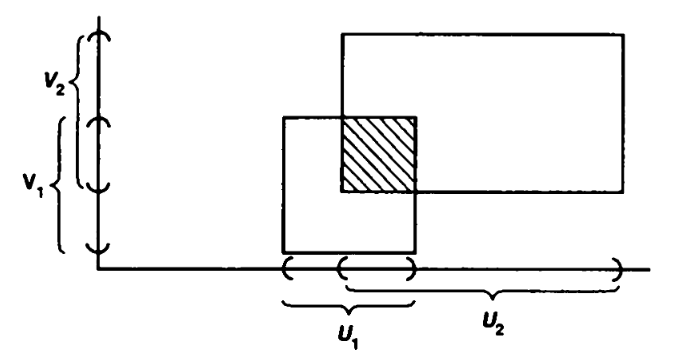
\includegraphics[scale=0.45]{../assets/product_topo.png}}
        \caption{}
        \label{fig:1}
    \end{figure}
\end{rem}

\begin{thm}
    If $\cal B$ is a basis for the topology of $X$ and $\cal C$ is the basis for the topology on $Y$, then the collection
    $$ \cal D = \{B \times C \mid B \in \cal B \text{ and } C \in \cal C\} $$ 
    is a basis for the topology of $X \times Y$.
\end{thm}
\begin{proof}
    Let $W$ be the open subset of $X \times Y$ which is the product topology hence by definition there exist $U \times V \in X \times Y$ such that $U$ is open in $X$ and $V$ is open in $Y$. Since $\cal B$ and $\cal C$ are the bases for topology on $X$ and $Y$ respectively there exists $B \in \cal B$ and $C \in \cal C$ such that for each $x \in U \implies x \in B \subset U$ and for each $y \in V \implies y \in C \subset V$. Therefore, $x \times y \in B \times C \subset U \times V$. Hence by lemma $3$, $\cal D$ is the basis for topology on $X \times Y$.    
\end{proof}

\begin{exer}
        
\end{exer}

\begin{defn}[Projections]
    Let $\pi_1 : X \times Y \to Y$ be defined by the equation
    $$ \pi_1(x,y) = x;$$ 
    let $\pi_2 : X \times Y \to Y$ be defined by the equation
    $$ \pi_2(x,y) = y.$$
    The maps $\pi_1$ and $\pi_2$ are called the {\bf projections} of $X \times Y$ onto $X$ and $Y$ respectively.
\end{defn}
\begin{rem}
    The maps $\pi_1$ and $\pi_2$ are surjective.
\end{rem}
If $U$ is an open set of $X$ then $\pi_1^{-1}(U) = U \times Y$ which is open is $X \times Y$. Similarly, $\pi_2^{-1}(V) = X \times V$ which is open in $X \times Y$.

\begin{thm}
    The collection
    $$ \cal S = \{\pi_1^{-1}(U) \mid U \text{ open in } X\} \cup \{\pi_2^{-1}(V) \mid V \text{ open in } Y\}$$
    is a subbasis for the product topology on $X \times Y$.
\end{thm}
\begin{proof}
    Let $S_{ij} = \pi_1^{-1}(U_i) \cup \pi_2^{-1}(V_j)$. To show that $\cal S$ is subbasis we need to show that $\cup_j(\cup_i S_{ij}) = X$. 
    
    \noindent $(\implies)$ Let $x \in S_{ij}$ implies that $x \in U_i \times Y$ or $x \in X \in V_j$. In either case, $x \in X \times Y$ since $U_i \subset X$ and $V_j \subset Y$. $\cup_j(\cup_i S_{ij}) \subset X \times Y$.

    \noindent $(\impliedby)$ Let $x \in X \times Y$. This case is trivial since $U_i = X$ and $V_j = Y$ and then $x \in (X \times Y) \cup (X \times Y)$. This implies that $x \in \cup_j(\cup_i S_{ij})$. Therefore, $\cup_j(\cup_i)S_{ij} = X \times Y$. 

    TODO
\end{proof}

\begin{defn}[Open map]
    A map $f : X \to Y$ is said to be an {\bf open map} if for every open set $U$ of $X$, the set $f(U)$ is open in $Y$.
\end{defn}

\begin{thm}
    The projection maps $\pi_1 : X \times Y \to X$ and $\pi_2 : X \times Y \to Y$ are open maps.
\end{thm}
\begin{proof}
    Let $U \times V$ be the open set in $X \times Y$ where $U$ is open is $X$ and $V$ is open in $Y$. Since, $\pi_1(U \times V) = U \subset X$ and $U$ is open in $X$. Same argument can be applied for $\pi_2(U \times V)$. This shows that $\pi_1$ and $\pi_2$ are open maps.
\end{proof}

\section{The Subspace topology}
\begin{defn}
    Let $X$ be a topological space with topology $\cal T$. If $Y$ is a subset of $X$, the collection
    $$ \cal T_Y = \{Y \cap U \mid U \in \cal T_X\} $$
    is a topology on $Y$, called the {\bf subspace topology}. With this topology, $Y$ is called the {\bf subspace} of $X$.
\end{defn}
It is easy to check that $\cal T$ is the topology with the fact that 
$$ \bigcup_{i \in I} U_i \cap Y = (\cup_{i \in I} U_i) \cap Y$$

\begin{lem}
    If $\cal B$ is a basis for the topology on $X$ then the collection 
    $$ \cal B_y = \{ B \cap Y \mid B \in \cal B\}$$
    is the basis for the subspace topology on $Y$.    
\end{lem}
\begin{proof}
    Given an open set $U \subset X$. For each $y \in U \cap Y$, since $U \cap Y \subset U$, there exists $B \in \cal B$ such that $y \in B \subset U \cap Y$. Also, $y \in Y$ hence
    $$
    \begin{array}{l}
        y \in B \cap Y \subset B \subset U \cap Y \\
        y \in B \cap Y \subset U \cap Y        
    \end{array} 
    $$
    By lemma $3$, the collection $\{B \cap Y \mid B \in \cal B\}$ is the basis for the subspace topology on $Y$.
\end{proof}
\begin{lem}
    Let $Y$ be a subspace of $X$. If $U$ is open in $Y$ and $Y$ is open in $X$, then $U$ is open in $X$.
\end{lem}
\begin{proof}
    Since $U \in Y$. We have 
    $$
    \begin{array}{l}
        U = \bigcup (U_x \cap Y) \\
        U = (\bigcup U_x) \cap Y \\        
    \end{array}
    $$
    Since, $U_x$'s are open in $X$ so do their arbitrary union and $Y$ is open in $X$. Finite intersection of open sets is open. Hence $U$ is open in $X$.
\end{proof}

\begin{thm}[Relationship between subspace and product topology]
    If $A$ is a subspace of $X$ and $B$ is a subspace of $Y$, then the product topology on $A \times B$ is the same as the topology $A \times B$ inherits as a subspace of $X \times Y$.
\end{thm}
\begin{proof}
    Let $\cal B$ be the basis of the product topology on $A \times B$. 
    $$ \cal B = \{U \times V \mid U \text{ in basis of } A; V \text{ in basis of } B\} $$
    and $\cal B'$ be the basis of the topology $A \times B$ inherits as a subspace of $X \times Y$.
    $$ \cal B' = \{(A \times B)\cap (U_x \times V_y) \mid U_x \times V_y \text{ in basis of } X \times Y\} $$
    We need to show that $\cal B = \cal B'$. 
    
    \noindent $(\implies)$ Since, $A$ is a subspace of $X$ and $B$ is a subspace of $Y$, implies $U = A \cap U_x$ where $U_x$ is in the basis of $X$ and $V = B \cap V_y$ where $V_y$ is in the basis of $Y$. Hence. 
    \begin{align*}
        U \times V &= (A \cap U_x) \times (B \cap V_y)\\
        U \times V &= (A \times B) \cap (U_x \times V_y)        
    \end{align*}
    Last equation can be seen by drawing the figure. Hence, $\cal B \subset \cal B'$.

    \noindent $(\impliedby)$ For any element $(A \times B) \cap (U_x \cap V_y)$ in $\cal B'$, it can be written as $(A \cap U_x) \times (B \cap V_y)$ (can be seen from visualization). Since $U_x$ is in the basis of $X$, $A \cap U_x$ is in the basis of $A$ as a subspace of $X$. Same argument can be extended for $B \cap V_y$.
    \begin{align*}
        (A \times B) \cap (U_x \cap V_y) &= U' \times V'\\
        (A \times B) \cap (U_x \cap V_y) &\in \cal B\\
        \cal B' &\subset \cal B
    \end{align*}
    where $U'$ and $V'$ are  some basis element of $A$ and $B$ respectively. Since, $\cal B = \cal B'$ hence the topology generated by them are equal.
\end{proof}

\begin{rem}
    Let $X$ be an ordered set in the order topology, and let $Y$ be a subset of $X$. Then order relation on $X$, when restricted to $Y$, makes $Y$ into an ordered set.    
\end{rem}
\begin{rem}
    However, the resulting order topology on $Y$ need not be the same as the topology that $Y$ inherits as a subspace of $X$.
\end{rem}

\begin{defn}[Convex set]
    Given an ordered set $X$, A subset $Y$ of $X$ is {\bf convex} in $X$ if for each pair of points $a < b$ of $Y$, the entire interval $(a,b)$ of $X$ is contained in $Y$. 
\end{defn}
\begin{rem}
    The interval and rays in $X$ are convex in $X$.    
\end{rem}
\begin{thm}
    Let $X$ be an ordered set in the order topology; let $Y$ be a subset of $X$ that is convex in $X$. Then the order topology on $Y$ is the same as topology $Y$ inherits as a subspace of $X$.
\end{thm}
\begin{proof}
    TODO
\end{proof}
\section{Closed set and Limit points}
\begin{defn}[Closed set]
    A subset $A$ of a topological space $X$ is said to be closed if the set $X - A$ is open.
\end{defn}
\begin{thm}
    Let $X$ be a topological space. Then the following conditions hold:
    \begin{enumerate}
        \item $\phi$ and $X$ are closed.
        \item Arbitrary intersections of closed sets are closed.
        \item Finite union of closed sets are closed.
    \end{enumerate}
\end{thm}
\begin{proof} \noindent
    \begin{enumerate}
        \item This is obvious.
        \item Let $\{U_\alpha\}_{\alpha \in I}$ is the collection of closed subset of $X$. Let $J \subset I$. We write $(\cap_{\alpha \in J}U_\alpha)^c = \cup_{\alpha \in J}U_\alpha^c$. Since each $U_\alpha$ is closed implies $U_\alpha^c$ is open and so their arbitrary union. This shows that $\cap_{\alpha \in J}U_\alpha$ is closed.
        \item We write $(\cup_{i=1}^n U_i)^c = \cap_{i = 1}^n U_i^c$. Since each $U_i$ is closed hence $U_i^c$ is open and so their finite intersection. This shows that $\cup_{i=1}^n U_i$ is closed.
    \end{enumerate}
\end{proof}
\begin{thm}
    Let $Y$ be a subspace of $X$. Then a set $A$ is closed in $Y$ if and only if it equals the intersection of a closed set of $X$ with $Y$.
\end{thm}
\begin{proof}
    TODO
\end{proof}
\begin{thm}
    Let $Y$ be a subspace of $X$. If $A$ is closed in $Y$ and $Y$ is closed in $X$, then $A$ is closed in $X$.
\end{thm}
\begin{proof}
    TODO
\end{proof}

\subsection{Closure and Interior of a set}
Given a subset $A$ of a topological space $X$, the {\bf interior} of a $A$ is defined as the union of all open sets contained in $A$, and the {\bf closure} of $A$ is defined as the intersection of all closed sets containing $A$.
$$ \text{Int}A \subset A \subset \bar{A} $$

\begin{rem}
    If $A$ is open, then $\text{Int}A = A$ and if $A$ is closed, then $\bar{A} = A$.
\end{rem}

\begin{thm}
    Let $Y$ be a subspace of $X$, let $A$ be a subset of $Y$, let $\bar{A}$ denote the closure of $A$ in $X$. Then the closure of $A$ in $Y$ equals $\bar{A} \cap Y$.
\end{thm}
\begin{proof}
    Let denote the closure of $A$ in $Y$ as $cl_Y(A)$ and $\bar{A}$ as closure of $A$ in $X$. Hence, $cl_Y(A) = \cap_{\alpha \in I} (U_X^\alpha \cap Y) = (\cap_{\alpha \in I}U_X^{\alpha}) \cap Y$ where each $U_X^\alpha \cap Y$ contains $A$ and is closed in $Y$ (which implies each $U_X^\alpha$ contains $A$ and is closed in $X$). Since, arbitrary intersection of closed set is closed. $\cap_{\alpha \in I}U_X^{\alpha}$ is $\bar{A}$ (by definition of closure).
\end{proof}

\begin{thm}[Closure in terms of basis]
    Let $A$ be a subset of the topological space $X$.
    \begin{enumerate}
        \item Then $x \in \bar{A}$ if and only if every open set containing $x$ intersects $A$.
        \item Supposing the topology of $X$ is given by a basis, then $x \in \bar{A}$ if and only if every basis element $B$ containing $x$ intersects $A$.
    \end{enumerate}
\end{thm}
\begin{proof}
    TODO
\end{proof}
\begin{rem}
    Consider the subspace $Y = (0,1]$ of the real line. The set $A = (0, \frac{1}{2})$ is a subset of $Y$, its closure in $\mathbb{R}$ is the set $[0, \frac{1}{2}]$, and its closure in $Y$ is the set $[0,\frac{1}{2}] \cap Y = (0,\frac{1}{2}]$.
\end{rem}

\begin{thm}
    Let $A$ be a subset of the topological space $X$.
    \begin{enumerate}
        \item Then $x \in \bar{A}$ if and only if every open set $U$ containing $x$ intersects $A$.
        \item Supposing the topology of $X$ is given by a basis, then $x \in \bar{A}$ if and only if every basis element $B$ containing $x$ intersect $A$.
    \end{enumerate}
\end{thm}
\begin{proof}
    $(1)$ The contrapositive of the statement is "$x \notin \bar{A}$ if and only if there exists an open set $U$ containing $x$ which does not intersects $A$." This is easy to show. This implies $x \in X - \bar{A}$ and $\bar{A}$ is closed in $X$ hence $U = X - \bar{A}$ is open in $X$ containing $x$.\\
    Conversely, let $U$ be an open set containing $x$ which does not intersect $A$. $X - U$ is closed set containing $A$ hence by definition of $\bar{A}$, $\bar{A} \subset X - U$. This implies $x \notin \bar{A}$.

    $(2)$ From $(1)$, we just have to show that every open set $U$ containing $x$ intersects $A$ if and only if every basis element $B$ containing $x$ intersects $A$. $(\implies)$ If every open set containing $x$ intersects $A$ then so does every basis element $B$ containing $x$ since basis elements are open. $(\impliedby)$ Every open set containing $x$ has to contain the basis elements containing $x$. Since these basis elements intersects $A$ which implies the open set containing them intersects $A$.
\end{proof}

\begin{defn}[Limit points]
    If $A$ is a subset of the topological space $X$ and if $x$ is a point of $X$, then $x$ is a {\bf limit point} of $A$ if every neighbourhood of $x$ intersects $A$ in some point other than $x$ itself.
    $$ x \in \overline{A-[x]}$$
\end{defn}
\begin{thm}
    Let $A$ be a subset of the topological space $X$, let $A'$ be the set of all limit points of $A$. Then
    $$ \bar{A} = A \cup A' $$
\end{thm}
\begin{proof}
    TODO
\end{proof}
\subsection{Hausdorff Spaces}
\begin{defn}[Hausdorff Space]
    A topological space $X$ is called a {\bf Hausdorff space} if for each pair $x_1, x_2$ of distinct points of $X$, there exists neighbourhood $U_1$ and $U_2$ of $x_1$ and $x_2$ respectively in $X$, that are disjoint.

    This is also known as $T$-$2$ separartion axiom.
\end{defn}
\begin{thm}
    Every finite point set in a Hausdorff space $X$ is closed.
\end{thm}
\begin{proof}
    
\end{proof}

\section{Continuous functions}
\begin{defn}[Continuous function]
    Let $X$ and $Y$ be topological spaces. A function $f : X \to Y$ is said to be continous if for each open subset $V$ of $Y$, the set $f^{-1}(V)$ is an open set of $X$.    
\end{defn}
If the topology on the range space $Y$ is given by the basis elements $\cal B$ then it is enough to show that the {\bf inverse image of the basis element is open}. Since open set $V$ in $Y$ is given by $ V = B_1 \cup B_2 \cup \dots$ and 
$$ f^{-1}(V) = f^{-1}(B_1) \cup f^{-1}(B_2) \cup \dots $$
each element of RHS is open hence their arbitrary union is also open.

If the topology on $Y$ is given by subbasis $\cal S$ then it is enough to show that {\bf inverse image of each element of subbasis is open}. Since an element $B$ of basis can be written as $S_1 \cap S_2 \cap \dots \cap S_n$.
$$ f^{-1}(B) = f^{-1}(S_1) \cap f^{-1}(S_2) \cap \dots \cap f^{-1}(S_n)$$
each element of RHS is open hence $f^{-1}(B)$ is open then from above paragraph, it implies that $f$ is continuous. 

\begin{exer}
    Prove that the $\varepsilon-\delta$ defintion of continuity for real-valued functions is equivalent to the above definition of continuity.
\end{exer}
\begin{sol*}
    ($\implies$) $\varepsilon-\delta$ implies the open ball definition.\\
    Let $f: \bb R \to \bb R$ be the continuous function hence for given $\varepsilon > 0$ there exists a $\delta > 0$ such that for some $x_0 \in \bb R$, $|f(x) - f(x_0)| < \varepsilon$ whenever $|x-x_0| < \delta$. Suppose $x \in \bb R$ such that $f(x) \in (f(x_0) - \varepsilon, f(x_0) + \varepsilon)$. This implies 
    $$ x \in f^{-1}(f(x_0) - \varepsilon, f(x_0) + \varepsilon) $$
    Then by $\varepsilon-\delta$ defintion of continuity, $x \in (x_0-\delta, x_0+\delta)$. This means $f^{-1}(f(x_0) - \varepsilon, f(x_0) + \varepsilon) \subset (x_0-\delta, x_0+\delta)$. For other way if $x \in (x_0-\delta, x_0+\delta)$ then by $\varepsilon-\delta$ defintion of continuity, $f(x) \in (f(x_0) - \varepsilon, f(x_0) + \varepsilon)$. Hence, $(x_0-\delta, x_0+\delta) \subset f^{-1}(f(x_0) - \varepsilon, f(x_0) + \varepsilon)$. 

    This equality implies that inverse image of the open set in range space $\bb R$ is open in domain space $\bb R$.

    $(\impliedby)$ If $f: \bb R \to \bb R$ is continuous then if $V$ is open in range space $\bb R$ then $U = f^{-1}(V)$ is open in domain space $\bb R$. For some $x_0 \in \bb R$ and given $\varepsilon > 0$, $V = (f(x_0)-\varepsilon, f(x_0)+\varepsilon)$ is open in $\bb R$. Since $U$ contians $x_0$, there exists a basis element $(a,b) \in \bb R$ such that $x_0 \in (a,b) \subset U = f^{-1}(V)$. We choose $\delta > 0$ as $\min\{x_0-a, x_0-b\}$ then $(x_0 - \delta, x_0+\delta) \subset U$ and whenever $|x-x_0| < \delta$ we have $|f(x) - f(x_0)| < \varepsilon$.
\end{sol*}
\begin{eg}
    If $f: \bb R \to \bb R_l$ is identity function then $f$ is not continuous since any open set $[a,b)$ (basis element of $\bb R_l$) containing $x$, its inverse image is $[a,b)$ which is not open in $\bb R$.
\end{eg}
\begin{eg}
    If $g: \bb R_l \to \bb R$ is identity function then $g$ is continuous since any open set $(a,b)$ containing $x$, its inverse image is $(a,b)$ which is open in $\bb R_l$. ($(a,b) = \cup_{n=1}^\infty[a+\frac{1}{n},b)$).
\end{eg}
\begin{thm}
    Let $X$ and $Y$ be topological spaces; let $f:X \to Y$. Then the following are equivalent:
    \begin{enumerate}
        \item $f$ is continuous.
        \item For every subset $A$ of $X$, one has $f(\bar{A})\subset \overline{f(A)}$.
        \item For every closed set $B$ of $Y$, the set $f^{-1}(B)$ is closed in $X$.
        \item For each $x\in X$ and each neighbourhood $V$ of $f(x)$, there is a neighbourhood $U$ of $x$ such that $f(U) \subset V$.
    \end{enumerate}   
    If the condition in $(4)$ holds for the point $x$ of $X$, we say that $f$ is continous at the point $x$.
\end{thm}
\begin{proof}
    $(1 \implies 2)$ TODO
\end{proof}

\subsection{Homeomorphism}
\begin{defn}[Homeomorphism]
    Let $X$ and $Y$ be the topological spaces; let $f : X \to Y$ be a bijection. If both the function $f$ and the inverse function $f^{-1}: Y \to X$ are continuous, then $f$ is called homeomorphism.
\end{defn}
Another way to define a homeomorphism is to say that it is a bijective correspondence $f: X \to Y$ such that $f(U)$ is open if and only if $U$ is open.
\begin{defn}[Topological properties]
    Any properties of $X$ that are entirely expressed in terms of the topology of $X$ (i.e. in terms of open sets of $X$) yields, via the correspondence $f$, the corresponding property for the space $Y$, called topological properties.
\end{defn}
\begin{defn}[Topological imbedding]
    Suppose that $f : X \to Y$ is an injective continuous map, where $X$ and $Y$ are topological spaces. Let $Z$ be the image set $f(X)$, considered as a subspace of $Y$; then the function $f' : X \to Z$ obtained by restricting the range of $f$, is bijective. If $f'$ is an homeomorphism of $X$ with $Z$, then map $f : X \to Y$ is  called a {\bf topological imbedding} of $X$ in $Y$.
\end{defn}
\begin{thm}[Constructing continuous functions]
    TODO
\end{thm}
\begin{thm}[Pasting lemma]
    Let $X = A \cup B$, where $A$ and $B$ are closed in $X$. Let $f \colon A \to Y$ and $g \colon B \to Y$ be continuous. If $f(x) = g(x)$ for every $x \in A \cap B$, then $f$ and $g$ combine to give a continuous function $h \colon X \to Y$, defined by setting $h(x) = f(x)$ if $x \in A$ and $h(x) = g(x)$ if $x \in B$.
\end{thm}
\begin{proof}
    Let $C$ be a closed set in $Y$. Then
    $$ h^{-1}(C) = f^{-1}(C) \cup g^{-1}(C).$$
    Since, $f$ and $g$ are continuous, $h^{-1}(C)$ is union of two closed set hence it is closed. Therefore, $h$ is continuous.
\end{proof}
\subsection{Quotient Topology}
\begin{defn}[Quotient map]
    Let $X$ and $Y$ be topological spaces; let $p : X \to Y$ be a surjective map. The map $p$ is said to be a {\bf quotient map} provided a subset $U$ of $Y$ is open in $Y$ if and only if $p^{-1}(U)$ is open in $X$.
\end{defn}
\begin{defn}[Quotient topology]
    If $X$ is a space and $A$ is a set and if $p : X \to A$ is a surjective map, then there exists exactly one topology $\cal T$ on $A$ relative to which $p$ is a quotient map; it is called the {\bf quotient topology} induced by $p$.
\end{defn}

The topology $\cal T$ is consists of those subsets $U$ of $A$ such that $p^{-1}(U)$ is open in $X$.

\begin{defn}[Quotient space]
    Let $X$ be a topological space, and let $X^*$ be a partition of $X$ into disjoint subsets whose union is $X$. Let $p : X \to X^*$ be the surjective map that carries each point of $X$ to the element of $X^*$ containing it. In the quotient topology induced by $p$, the space $X^*$ is called a {\bf quotient space} of $X$.
\end{defn}
A subset $U$ of $X^*$ is a collection of equivalence classes, and the set $p^{-1}(U)$ is the union of the elements of $X$ whose equivalence classes belong to $U$. Thus, open set of $X^*$ is a collection of equivalence classes whose union is an open set of $X$.

\begin{thm}
    Let $p : X \to Y$ be a quotient map; let $A$ be a subspace of $X$ that is saturated with respect to $p$; let $q : A \to p(A)$ be the map obtained by restricting $p$.
    \begin{enumerate}
        \item If $A$ is either open or closed in $X$, then $q$ is a quotient map.
        \item If $p$ is either an open map or a closed map, then $q$ is a quotient map.
    \end{enumerate}
\end{thm}
\begin{proof}
    TODO.
\end{proof}

\subsection{Topological Groups}
\begin{defn}[Topological Group]
    A {\it topological group} $(G,\cdot,\cal T)$ consists of group $(G,\cdot)$ and a topology $\cal T$ on $G$ for which the multiplication map
    $$
    \begin{aligned}
        G \times G &\to G \\
        (g,h) &\mapsto g \cdot h = gh
    \end{aligned} 
    $$
    and the inversion map
    $$
    \begin{aligned}
        G &\to G \\
        g &\mapsto g^{-1}
    \end{aligned} 
    $$
    are continuous. We call $\cal T$ to be {\it group topology} on $G$. We can combine these two conditions as:
    $$
    \begin{aligned}
        \kappa \colon G \times G &\to G \\
        (g,h) &\mapsto g^{-1}h
    \end{aligned} 
    $$
    If $G$ is a topological group then $\kappa$ is continuous.
\end{defn}
Conversely, if $\kappa$ is continuous, then the maps $g \mapsto g^{-1} = \kappa(g,e)$ and $(g,h) \mapsto gh = \kappa(\kappa(g,e),h)$ are continuous (composition of continuous maps).

\begin{thm}
    Suppose that $G$ is a topological group. For every $a \in G$, the {\it right tranlation map}
    $$ \rho_a(g) = ga$$
    the {\it left tranlation map}
    $$ \lambda_a(g) = ag$$
    and the {\it conjugation map}
    $$ \gamma_a(g) = aga^{-1}$$
    are homeomorphisms of $G$ onto itself, with inverses $\lambda_{a^{-1}}$, $\rho_{a^{-1}}$, $\gamma_{a^{-1}}$, respectively.
\end{thm}
\begin{proof}
    We will show it from $\rho_a$ rest all will follow the same.\\
    Injectivity is trivial from group operation right cancellation. For surjectivity, let $g \in G$ then there exists $ga^{-1}\in G$ such that $\rho_a(ga^{-1}) = g$. Hence, it is surjective.

    Let $U \in G$ be an open subset. 
    $$ (\rho_a)^{-1}(U) = \{g \in G \colon \rho_a(g) \in U\} = Ua^{-1}$$
    Since, $U = Ua^{-1}a$ is open in $G$ and multiplication map $G \times G \to G$ is continuous implies that inverse image of $Ua^{-1}a \in G$ which is $(Ua^{-1},a) \in G \times G$ is open. Hence, $Ua^{-1}$ is open in $G$ (product topology). This shows that $\rho_a$ is continuous and since $a$ is arbitrary, we can choose $(\rho_a)^{-1}$ as $\rho_{a^{-1}}$(inverse map is also continuous then). This also shows that $\rho_a$ is homeomorphism.

    Similarly, for other two maps, it can be shown that they are homeomorphism from $G \to G$.
\end{proof}

\begin{thm}
    A topological group $G$ is Hausdorff if and only if some singleton $\{a\} \subset G$ is closed.
\end{thm}
\begin{proof}
    $(\implies)$ Assume $G$ is Hausdorff, to show that $\{a\}^c$ is open. For all $b(\neq a) \in G$, there exists open nbd $U_b, U_a\in G$ such that $b \in U_b$ and $a \in U_a$ and they are disjoint. Therefore, $\bigcup\limits_{\substack{b\in G \\ b \neq a}} U_b = G\backslash\{a\} = \{a\}^c$ which is open. (Hausdorff implies $T$-1 means singletons are closed.)

    \noindent $(\impliedby)$ Assume $\{a\} \in G$ is closed. Take the inverse image of $\{a\}$ under the continuous map $(g,h) \mapsto g^{-1}ha$. $g^{-1}ha = a \implies g = h$. Hence, the inverse image is $\Delta = \{(g,g) \colon g \in G\}$ which is closed in $G \times G$ ($\because$ map is continuous) which means $G$ is Hausdorff. ($\Delta$ is closed in $G \times G$ implies $G$ is Hausdorff; $\Delta^c$ is open then the open nbd for each point $(x,y), x \neq y$ is basis elements of $G \times G$ and intersection of those basis elements has to be empty otherwise $(z,z) \in \Delta^c$, $z$ in intersection, which is not possible).
\end{proof}

\subsection{Quotients}

Suppose $H$ is a subgroup of a topological group $G$. We endow the set $G/H$ of left cosets with the quotient topology w.r.t natural map
$$ p \colon G \to G/H, \qquad g \mapsto gH.$$
Thus a subset of $G/H$ is open if and only if its $p$-preimage is open.

\begin{prop}
    Let $G$ be a topological group and let $H$ be a subgroup. Then the quotient map
    $$ p \colon G \to G/H$$
    is open. The quotient $G/H$ is Hausdorff if and only if $H$ is closed in $G$.
\end{prop}
\begin{proof}
    TODO
\end{proof}
\section{Compactness}
\begin{defn}[Covering]
    A collection $\cal A$ of subsets of a space $X$ is said to cover $X$, or to be a {\it covering} of $X$, if the union of the elements of $\cal A$ is equal to $X$. It is called {\it open covering} of $X$ if its elements are open subsets of $X$. 
\end{defn}
\begin{defn}[Compact space]
    A space $X$ is said to be {\it compact} if every open covering $\cal A$ of $X$ contains a finite subcollection that also covers $X$.
\end{defn}
\begin{rem}
    If $Y$ is a subspace of $X$, a collection $\cal A$ of subsets of $X$ is said to cover $Y$ if the union of its elements {\bf contains} $Y$.
\end{rem}
\begin{lem}
    Let $Y$ be a subspace of $X$. Then $Y$ is compact if only if every covering of $Y$ by sets open in $X$ contains a finite subcollection covering $Y$.
\end{lem}
\begin{proof}
    $(\implies)$ Assume $Y$ is compact and $\{A_\alpha\}_{\alpha \in I}$ be the cover of $Y$ by open sets of $X$. Then the collection $\{A_\alpha \cap Y\}_{\alpha \in I}$ of open sets of $Y$ covers $Y$. Since $Y$ is compact, the finite subcover of $Y$ by open sets of $Y$ is $\{A_1\cap Y, \dots, A_n \cap Y\}$. Hence $\{A_1, \dots, A_n\}$ is the finite subcover of $Y$ by open sets of $X$. 

    \noindent $(\impliedby)$ Let $\{A_\alpha\}_{\alpha \in I}$ be the collection of open sets in $X$ that covers $Y$. Then $\{A_\alpha \cap Y\}_{\alpha \in I}$ is a covering of $Y$ by open sets of $Y$. By hypothesis, there exists a finite subcovering of $Y$ by open sets of $X$, $\{A_1, \dots, A_n\}$. Hence, $\{A_1 \cap Y, \dots, A_n \cap Y\}$ is finite subcover of $Y$ by open sets in $Y$. Therefore, $Y$ is compact.
\end{proof}

% \begin{



\subsection{Limit Point Compactness}
\begin{defn}[Limit point compact]
    A space is said to be {\it limit point compact} if every infinite subset of $X$ has a limit point.

    This is also referred as {\it Frechet compactness} or {\it Bolzano-Weierstrass property}.
\end{defn}
\begin{thm} \label{23}
    Compactness implies limit point compactness, but not conversely.
\end{thm}
\begin{proof}
    Let $X$ be compact space. We need to show that every infinite subset $A \subset X$ has a limit point. We will prove contrapositive: If $A$ has no limit point then $A$ must be finite.
    
    Since $A$ does not have limit point implies $A$ contains all its limit points. Therefore, $A$ is closed. For any $a \in A$, any neighbourhood $U$ of $a$ intersect $A$ at point $a$ only. Hence $\{X - A, \{U_a\}_{a\in A}\}$ is an open cover of $X$ and since $X$ is compact, it has finite subcover, say $\{X - A, U_1, U_2, \dots, U_n\}$. Since, $X - A$ does not intersect $A$ and each $U_a$ cover only $a \in A$ hence $A$ has to be finite. 
\end{proof}
\begin{eg}[Counter example of converse statement]
    Let $Y$ consist of two points, give $Y$ the trivial topology. Then the space $ X = \bb Z_+ \times Y$ is limit point compact, for every non empty subset of $X$ has a limit point. It is not compact since the cover $\{U_n\}_{n \in \bb Z_+} = \{n\} \times \{a,b\}$ does not have any finite subcover.
\end{eg}

\subsection{Sequential Compactness}
\begin{defn}[Sequential Compactness]
    Let $X$ be topological space. If $(x_n)$ is a sequence of point of $X$, and if $n_1 < n_2 < \dots < n_i < \dots $ is an increasing sequence of positive integers, then the sequence $(y_i)$ defined by setting $y_i = x_n$ is called a subsequence of the sequence $(x_n)$. The space $X$ is said to be {\bf sequentially compact} if every sequence of points of $X$ has a convergent subsequence.
\end{defn}
\begin{thm}
    Let $X$ be a metrizable space. Then the following are equivalent:
    \begin{enumerate}
        \item $X$ is compact.
        \item $X$ is limit point compact.
        \item $X$ is sequentially compact.
    \end{enumerate}
\end{thm}
\begin{proof}
    $(1 \implies 2)$ is already done in previous theorem \ref{23}. \\
    $(2 \implies 3)$ Assume $X$ is limit point compact. Let $(x_n)$ be a sequence in $X$, consider the set $A = \{x_n \mid n \in \bb Z_+\}$. 
    
    \noindent \underline{Case 1:} If $A$ is finite then there exists a $N$ and $x \in X$ such that for all $n > N$, $x_n = x$. Hence, the subsequence can be constant sequence and that converges trivially.

    \noindent \underline{Case 2:} If $A$ is infinite then it has a limit point (since $X$ is limit point compact). Construct a subsequence as follows: 
    $$ x_1 \in B(x,1), \qquad x_{n_k} \in B(x,1/n_k)$$
    for $1 < n_k < n_{k+1} < \dots$ and such a $x_{n_k}$ exists as $x$ is the limit point hence any neighbourhood around it contains infinite many point of $A$. This subsequence converges to $x$. Therefore, $X$ is sequentially compact. \\
    $(3 \implies 1)$ TODO
\end{proof}


\subsection{Local Compactness}
\begin{defn}[Locally compact]
    A space $X$ is said to be locally compact at $x$ if there is some compact subspace $C_x$ of $X$ and an open set $U_x$ of $X$ such that $x \in U_x \subset C_x$. If $X$ is locally compact at each of its points, $X$ is said simply to be locally compact.
\end{defn}
\begin{thm}
    Let $X$ be a space. Then $X$ is locally compact Hausdorff if and only if there exists a space $Y$ satisfying the following conditions:
    \begin{enumerate}
        \item $X$ is a subspace of $Y$.
        \item The set $Y-X$ consists of a single point.
        \item $Y$ is a compact Hausdorff space.
    \end{enumerate}
    If $Y$ and $Y'$ are two spaces satisfying these conditions, then there is a homeomorphism of $Y$ with $Y'$ that equals the identity map on $X$.
\end{thm}
\begin{proof}
    First, check the uniqueness. Let $Y$ and $Y'$ be two spaces satisfying these conditions. Define $h:Y \to Y'$. $h$ is identity on $X$ and it maps unique point of $Y-X$ to unique point of $Y'-X$. It is injective, surjective. For continuity, if $U \subset X \subset Y'$ then $h^{-1}(U)$ is open in $X \subset Y$(identity). For $U = \{\infty\} \subset Y'$ which is closed, $h^{-1}(U) = \{\infty'\} \subset Y$ which is closed in $Y$ since $Y$ is Hausdorff (singletons are closed in Hausdorff spaces). By symmetry, $h^{-1}$ is also continuous.

    \noindent$(\implies)$ Now, we assume that $X$ is locally compact and Hausdorff and construct $Y = X \cup \{\infty\}$ where $\infty$ is a symbol for the extra element. The topology $\cal T_Y$ on $Y$ is given by $(1)$ open sets of $X$ $(2)$ all sets of the form $Y - C$ where $C$ is a compact subspace of $X$. We need to check if this collection forms a topology or not. 
    \begin{enumerate}
        \item $(1)$ $\phi$ is in $X$ implies it is in the collection. $(2)$ since $\phi$ is compact in $X$ hence $Y - \phi = Y$ is in the collection. 
        \item  For arbitrary collection of open sets, there are three choices: $(1)$ $\cup U_\alpha$, where $U_\alpha$ is open in $X$ for each $\alpha$, should lie in $\cal T_Y$ (trivially lies in $\cal T_Y$). $(2)$ $\cup\{Y - C_\beta\}$ should lie in $\cal T_Y$ ($\cup\{Y - C_\beta\} = \{Y - \cap C_\beta\} = \{Y - C'\} \in \cal T_Y$) ({\bf since arbitrary intersection of compact set is compact}).  $(3)$ arbitrary collection of open sets of type $(\cup U_\alpha) \bigcup (\cup \{Y - C_\beta\})$ should lie in $\cal T_Y$ therefore, 
        $$ (\cup U_\alpha) \bigcup (\cup \{Y - C_\beta\}) = U \bigcup \{Y - C'\} = U \bigcup \{X - C'\}$$ 
        is open in $X$ since $C'$ is compact in $X$ hence closed ($X$ is Hausdorff), $X - C'$ is open and $U$ is open in $X$. Hence this is of type $(1)$ set implies lies in $\cal T_Y$.
        \item For finite intersection of open sets: $(a)$ trivial for open sets of type $(1)$ which are open in $X$. $(b)$ $\cap_{i=1}^n \{Y - C_i\} = Y - \cup_{i=1}^n C_i = Y - C'$ is of type $(2)$ since {\bf finite union of compact sets is finite}. $(c)$ $U_1 \cap \{Y - C\} = U_1 \cap \{X - C\}$ is open in $X$ hence its open in $Y$ (since $C$ is compact and hence closed in $X$). Given collection is a topology on $Y$.
    \end{enumerate}
    Now, we show that {\bf $X$ is a subspace of $Y$}. For this, we need to show that any open set of $X$ can be written as intersection of open set of $Y$ and $X$. This can be achieved by taking type $(1)$ sets and their intersection with $X$. Other direction, intersection of any open set of $Y$ with $X$ is open in $X$. If open set of $Y$ is of type $(1)$ then it is trivially open in $X$, if it is type $(2)$ then $\{Y - C\} \cap X = \{X - C\} \cap X = X - C$ which is open in $X$ since $C$ is compact in $X$ (Hausdorff).

    \noindent $Y - X$ is singleton by construction.

    \noindent {\bf To show $Y$ is compact and Hausdorff.} Let $\{A_\alpha\}_{\alpha \in I}$ is an open cover of $Y$. Then $\{A_\alpha \cap X\}_{\alpha\in I}$ is an open cover of $X$ which implies it cover $C \subset X$ which is compact in $X$. Therefore, $\{Y - C, \{A_\alpha \cap X\}_{\alpha \in I}\}$ is an open cover of $Y$. There will exist a $Y - C$ since $\{\infty\}$ is not contained in $X$. Since $C$ is compact there exists a finite subcover of $C$ which implies $\{\{A_1 \cap X, A_2 \cap X, \dots, A_n \cap X\}, Y - C\}$ is a finite cover of $Y$. Hence, $Y$ is compact.

    \noindent For any $x,y \in Y$, if both of lie in $X$ then there exists disjoint open sets in $X$ containing them since $X$ is Hausdorff. If one of them is $\{\infty\}$ then take compact set $C_x$ containing $x$ which contains an neighbourhood of $x$ and $Y - C_x$ is open in $Y$ containing the other point, both are disjoint. Hence, $Y$ is Hausdorff.

    \noindent $(\impliedby)$ Since $Y$ is Hausdorff and $X$ is a subspace of $Y$ hence it is Hausdorff (open neighbourhood in $Y$ intersection with $X$ are open in $X$). For any point $x \in X \subset Y$ there exists disjoint open sets $U$ and $V$ containing $x$ and single point of $Y - X$ respectively. $Y - V$ is closed and hence compact (since $Y$ is compact) which lies in $X$ (since $\{\infty\}$ is not in it) hence it is compact in $X$. Therefore, $X$ is locally compact.
\end{proof}

\begin{rem}
    If $X$ itself is compact then $Y$ is not very interesting space since $\{\infty\}$ is just an isolated point added to $X$. But if $X$ is not compact then any open neighbourhood around $\{\infty\}$ must intersect $X$ at some point other than $\{\infty\}$ otherwise that neighbourhood will just be $\{\infty\}$ which is not even open. This also shows that $\{\infty\}$ is the limit point of $X$ and $\overline{X} = Y$.
\end{rem}

\begin{defn}[One-point compactification]
    If $Y$ is compact Hausdorff space and $X$ is a proper subspace of $Y$ whose closure equals $Y$, then $Y$ is said to be a {\it compactification} of $X$. If $Y-X$ equals a single point, then $Y$ is called the {\it one-point compactification} of $X$.
\end{defn}

\begin{rem}
    We have shown in theorem $23$ that $X$ has a one point compactification $Y$ if and only if $X$ is locally compact Hausdorff and not itself compact. $Y$ is uniquely determined upto homeomorphism (if there are two one point compactification $Y$ and $Y'$ then they are homeomorphic to each other). 
\end{rem}
\begin{thm}
    Let $X$ be a Hausdorff space. Then $X$ is locally compact if and only if given in $x$ in $X$, and given a neighbourhood $U$ of $x$, there is a neighbourhood $V$ of $x$ such that $\overline{V}$ is compact and $\overline{V} \subset U$.
\end{thm}
\begin{proof}
    $(\impliedby)$ We need to show $X$ is locally compact. Let $C = \overline{V}$. Then we have $x \in V \subset \overline{V}$. $X$ is locally compact.
    
    \noindent $(\implies)$ Assume $X$ is locally compact. Then there exists compact and Hausdorff space $Y$ such that $X$ is subspace of $Y$ and $Y - X$ is singleton. Let $U$ be the neighbourhood of $x$ in $X$. Let $C = Y - U$. $C$ is closed in $Y$ (since $U$ is open in $Y$). $C$ is compact in $Y$ (since $Y$ is compact). Since $Y$ is Hausdorff, we can choose two disjoint open neighbourhoods $V$ and $W$ of $Y$ such that $x \in V$ and $C \subset W$. $\overline{V}$ is closed in $Y$ hence compact. Also, $\overline{V} \cap C = \phi$.
    
    Suppose for contradiction, $\overline{V} \cap C = \{y\}$, then $y$ has to be limit point of $V$ otherwise there is a contradiction with $V \cap W = \phi$. Since $y$ is limit point of $V$, let $U_y$ be a neighbourhood around $y$, $U_y \cap V\backslash\{y\} \neq \phi$. And $\{y\} \in C \subset W$ and $W$ is open hence $U_y \subset W$, which leads to contradiction to $V \cap W = \phi$. Hence $\overline{V} \cap C = \phi$.

    \noindent Therefore, $\overline{V} \subset U$.
\end{proof}
\begin{thm}
    Let $X$ be a locally compact Hausdorff; let $A$ be a subspace of $X$. If $A$ is closed in $X$ or open in $X$, then $A$ is locally compact.
\end{thm}
\begin{proof}
    Let $X$ be a locally compact Hausdorff space. For any $x \in X$ and an open neighbourhood $U$ of $x$, there exists an open neighbourhood $V$ of $x$ such that $\overline{V} \subset U$ and $\overline{V}$ is compact (from question $1$). Let $A \subset X$ be {\bf open} in $X$. Take arbitrary $x \in A$ and an open neighbourhood $U \cap A$ of $x$ which is open in $A$ (since $U$ is open in $X$). Also, $U \cap A$ is open in $X$ (both $U$ and $A$ are open in $X$). This implies $U \cap A$ is open in $Y$($=X \cup \{\infty\}$). Let $C = Y - (U \cap A)$, it is closed in $Y$ hence compact. Since $Y$ is Hausdorff, there exists an open set $V$ and $W$ in $Y$ containing $x$ and $C$, respectively such that $V \cap W = \phi$ which implies $\overline{V} \cap C = \phi$ (argument for this is in question $1$). Therefore, $\overline{V} \subset U \cap A$ and since $\overline{V}$ is closed in $Y$ hence compact in $Y$ implies compact in $X$ (since $X$ is subspace of $Y$). Since, $x \in A$ is arbitrary, from question $1$ we have $A$ is locally compact.

    Let $A \in X$ be closed. Since, $X$ is locally compact. For each $x \in X$ there exists a compact set $C_x$ containing $x$ and its neighbourhood $U_x$. Since, $C_x \cap A$ is closed in $C_x$, its compact in $C_x$ which implies it is compact in $X$ (in subspace topology). Also, $U_x \cap A$ is open in $A$ (subspace topology) and contained in $C_x \cap A$ (since $U_x \subset C$). Hence, $A$ is locally compact.
\end{proof}

\begin{cor}
    A space is $X$ is homeomorphic to an open subspace of a compact Hausdorff space if and only if $X$ is locally compact Hausdorff.
\end{cor}
\begin{proof}
    TODO
\end{proof}

\section{Connectedness}
\begin{defn}({\bf Separartion})
    Let $X$ be a topological space. A separartion of $X$ is a pair $U$, $V$ of disjoint nonempty open subsets of $X$ whose union is $X$. The space $X$ is said to be connected if there does not exist a separartion of $X$. OR

    A space $X$ is connected if and only if the only subsets of $X$ that are both open and closed in $X$ are the empty set and $X$ itself.
\end{defn}

\noindent For a subspace $Y$ of a topological space $X$:
\begin{lem}
    If $Y$ is a subspace of $X$, a separartion of $Y$ is a pair of disjoint nonempty sets $A$ and $B$ whose union is $Y$, neither of which contains a limit point of the other. The space $Y$ is connected if there exists no separartion of $Y$.
\end{lem}

\begin{proof}
    $(\implies)$ Let $Y$ has a separartion, say $A, B$, such that $A \cup B = Y$, $A \cap B = \phi$ and $A, B$ both are clopen in $Y$. \\
    \underline{Claim:} Neither $A$ nor $B$ contains the limit point of the other.
    Suppose for contradiction, $A$ contains the limit point of $B$ say $x$. Let $U$ be the neighbourhood of $x$. Then
    $$ U\backslash\{x\} \cap B \neq \phi$$
    and $A$ is open hence it contains $U$. Therefore, it contradicts that $A \cap B = \phi$. This shows $A$ does not contains the limit point of $B$. Similarly, we can exchange $A$ and $B$ in above argument to show that $B$ does not contains the limit point of $A$.

    \noindent $(\impliedby)$ Given disjoint subsets $A$ and $B$ of $Y$ such that $A \cup B = Y$ and neither of them contains the limit point of the other.\\ \underbar{Claim:} {\bf $A$ and $B$ are separartion of $Y$ ($A$ and $B$ are clopen in $Y$).} \\
    Since, $A \cap B = \phi$ and neither of them contains the limit point of the other implies that $\overline{A} \cap B = \phi$ and $\overline{B} \cap A = \phi$ ($\overline{A}$ and $\overline{B}$ are closure of $A$ and $B$ in $X$, respectively). $\overline{A} \cap Y = \overline{A} \cap (A \cup B) = (\overline{A} \cap A) \cup (\overline{A} \cap B) = A$. Similarly, $\overline{B} \cap Y = B$. Hence, closure of $A$ in $Y$ is $A$ and same for $B$ which implies $A$ and $B$ closed in $Y$. Since, $Y - A = B (\because A \cup B = \phi)$ which is closed implies $A$ is clopen and similarly $B$ is clopen. 
\end{proof}

\begin{eg}
    \begin{enumerate}
    \item Any set with trivial topology is trivially connected.
    \item Let $Y = [-1, 0) \cup (0,1]$ as a subspace of $\bb R$. $[-1, 0)$ and $(0,1]$ both are clopen in $Y$ and form the separartion of $Y$. Neither of the set contain the limit point of the other.
    \item Let $X$ be the subspace $[-1,1]$ of real line. $[-1, 0]$ and $(0,1]$ are disjoint and nonempty, but they do not form a separation of $X$ since $[-1,0]$ is not open in $X$. Also, it contains $0$, limit point of other set. There exists {\it no} separartion of $X$.
    \item Rationals $\bb Q$ are not connected. {\bf Only connected subspaces of $\bb Q$ are singletons. Hence, it is totally disconnected.} \underline{Proof:} If $Y$ is a subspace of $\bb Q$ containing two point $p$ and $q$. Then we can find a irrational number $a$ between them (density of irrationals) and then $Y \cap (-\infty, a) \cup Y \cap (a, \infty)$ is a separartion of $Y$. 
    \end{enumerate}
\end{eg}
\begin{lem}
    If the sets $C$ and $D$ form a separartion of $X$, and if $Y$ is a connected subspace of $X$, then $Y$ lies entirely within either $C$ or $D$.
\end{lem}
\begin{proof}
    Suppose for contradiction that $Y$ does not lie entirely in $C$ or $D$. $Y \cap C$ and $Y \cap D$ is nonempty. Since $C \cup D = X$, we have $(Y \cap C) \cup (Y \cap D) = Y$. Also, $C$ and $D$ are clopen subspace of $X$ hence $Y \cap C$ and $Y \cap D$ are clopen subspace of $Y$. They form a separation of $Y$ which is a contradiction to the fact that $Y$ is connected. Therefore, either $Y \cap C$ or $Y \cap D$ is empty.
\end{proof}
\begin{thm}
    The union of a collection of connected subspaces of $X$ that have a point in common is connected.
\end{thm}
\begin{proof}
    Let $\{A_\alpha\}$ be the collection of the connected subspaces of $X$ such that $\bigcap A_\alpha = p$. \underbar{Claim:} $Y = \bigcup A_\alpha$ is connected. \\ Suppose for contradiction $Y = C \cup D$ be a separartion of $Y$. $p$ will lie in one of them. WLOG, $p \in C$ implies $A_\alpha \subset C$ for all $\alpha$ since $p$ is common point in all of them implies $\bigcup A_\alpha\subset C$. This contradicts the fact that $D$ is nonempty. Therefore, $Y$ is connected. 
\end{proof}
\begin{thm}
    Let $A$ be a connected subspace of $X$. If $A \subset B \subset \overline{A}$, then $B$ is also connected. OR \\
    If $B$ is formed by adjoining to the connected subspace $A$, some or all of its limit points, then $B$ is connected.
\end{thm}
\begin{proof}
    Let $B = C \cup D$ be a separartion of $B$. $A \subset C \cup D$. Since, $A$ is connected implies $A \subset C$ or $D$. WLOG, assume $A \subset C$. Then $\overline{A} \subset \overline{C}$. Since $\overline{C} \cap D = \phi$ implies that $B$ cannot intersect with $D$. Hence $D$ is empty which is a contradiction.
\end{proof}
\begin{thm}
    The image of a connected space under a continuous map is connected.
\end{thm}
\begin{proof}
    Let $A$ be a connected set and $f \colon A \to B$ be a continuous map. It suffices to prove for the surjective continuous map.\\
    \underline{Claim:} $f(A)$ is connected.\\
    Let $f(A) = C \cup D$ be a separartion of $f(A)$. $f^{-1}(C)$ and $f^{-1}(D)$ are clopen in $A$ since $f$ is continuous. Also, $f^{-1}(C \cup D) = A$ and $f^{-1}(C) \cap f^{-1}(D) = \phi$. This forms a separartion of $A$ which contradicts the fact that $A$ is connected. Hence, $f(A)$ is connected.
\end{proof}
\begin{thm}
    A finite cartesian product of connected spaces is connected.
\end{thm}
\begin{proof}
    Let $\{A_1, A_2,\dots, A_n\}$ be a finite collection of connected sets. \\
    \underline{Claim:} $Y = A_1 \times A_2 \times \dots \times A_n$ is connected. \\
    Let $Y = C \cup D$. Let ${\bf x} = (x_1, \dots, x_n) \in Y$ implies ${\bf x}$ lies in either $C$ or $D$. WLOG, ${\bf x} \in C$. Since, $x_1 \in A_1$ implies $A_1 \times x_2 \dots \times x_n \subset C$, $x_2 \in A_2$ implies $x_1 \times A_2 \dots \times x_n \subset C$ and so on. Since ${\bf x}$ is arbitrary, we have $A_1 \times \dots \times A_n$ lies in $C$ and $D$ is empty which is a contradiction. Hence, $Y$ is connected.

    There is one more argument for this, $T$ argument. By showing it for product of two connected sets which involves the fact that union of two connected sets is connected if they have a point in common. Then use that $A_1 \times \dots \times A_n$ is homeomorphic to $(A_1 \times \dots \times A_{n-1}) \times A_n$ in induction.
\end{proof}
\begin{defn}[Path Connectedness]
    Given points $x$ and $y$ of the space $X$, a {\bf path} in $X$ from $x$ to $y$ is a continuous map $f \colon [a,b] \to X$ of some closed interval in the real line into $X$ such that $f(a) = x$ and $f(b) = y$.

    A space is said to be path connectedness if every pair of points of $X$ can be joined by a path in $X$.
\end{defn}
\begin{thm}
    A space $X$ is path connected then it is connected.
\end{thm}
\begin{proof}
    Let $X = C \cup D$ be a separartion of $X$. Let $x,y \in X$ are the two points then there exists a continuous map $f\colon [a,b] \to X$ such that $f(a) = x$ and $f(b) = y$. Since $[a,b]$ is connected, $f([a,b])$ is also connected (continuous image of a connected set is connected). Hence, $f([a,b])$ have to lie in either $C$ or $D$. Let $x \in C$ and $y \in D$ then $f([a,b])$ have to lie in either $C$ or $D$ but this is a contradiction since $f(a) = x$ is in $C$ and $f(b) = y$ is in $D$. Therefore, any one of the $C$ or $D$ has to be empty which shows $X$ is connected.

    A {\bf second proof} for this theorem is: "All roads lead to Rome". Let $x \in X$ be any point in a path connected space. Then for any $y \in X$, there exists a path $p_y \colon [a,b] \to X$ that connects $x$ and $y$ implies $X = \bigcup_{y \in X} p_y([a,b])$. Since $p_y$'s are continuous and each $p_y$ is connected (continuous image of a connected set $[a,b]$) with $x$ in common, we have their union ($X$) is connected. (Union of connected sets with a point in common is connected, previous theorem).
\end{proof}

\begin{rem}
    The converse does not hold. A connected space does not have to be path connected.
\end{rem}
\paragraph{{\bf Examples of path connected spaces:}}
\begin{enumerate}
    \item {\bf Unit ball} in $\bb R^n$ is path connected. $B^n \colon=\{\bf{x} \mid \|x\|_2 \leq 1\}$. Given any two point, we have a {\it straight line} path, defined as $f\colon[0,1] \to \bb R^n$ such that $f(t) = (1-t){\bf x} + t{\bf y}$.
    $$ \|f(t)\| = \|(1-t){\bf x} + t{\bf y}\| \leq (1-t)\|{\bf x}\| + t\|{\bf y}\| \leq 1(TODO)$$

    A similar argument shows that every open ball $B({\bf x},\epsilon)$ and every closed ball $\overline{B}({\bf x},\epsilon)$ in $\bb R^n$ is path connected.
    \item {\bf Punctured euclidean space}: $\bb R^n - \{0\}$. If $n > 1$, this space is path connected. Given any two point, there exists a straight line path or if $0$ is in between then take a point $z$ and take a broken path.
    
    For $n = 1$, there does not exists a path between $-1$ and $1$. Hence, is it not path connected.
    \item {\bf Unit Sphere} $S^{n-1}$ in $\bb R^n$ is given by the equation $ S^{n-1} = \{{\bf x} \mid \|x\| = 1\}$. If $n > 1$, it is path connected. For the map $g \colon \bb R^n - \{0\} \to S^{n-1}$ defined by $g({\bf x}) = {\bf x}\backslash\|x\|$ is continuous and surjective; and continuous image of a path connected space is path connected.(TODO: Proof)
\end{enumerate}
\paragraph{{\bf Example of connected spaces which are not path connected}}
TODO

\begin{defn}[Connected components]
    Given $X$, define an equivalence relation on $X$ by setting $x \sim y$ if there is a connected subspace of $X$ containing both $x$ and $y$. The equivalence classes are called the {\bf connected components} of $X$.
\end{defn}

\begin{thm}
    The components of $X$ are connected disjoint subspaces of $X$ whose union is $X$, such that each non empty connected subspaces of $X$ intersects only one of them.
\end{thm}
\begin{proof}
    Since components of $X$ are equivalence classes hence they are disjoint and their union is $X$. Let $A \subset X$ be a non empty connected subset. \underline{Claim:} $A$ intersects only one of the components. Let $C_1$ and $C_2$ be the components of $X$ and $A$ intersects them at points $a$ and $b$. Since, $a \in C_1 \cap A$ hence $A \cup C_1$ is connected set containing $a$ (union of connected sets with a point in common) and all elements of $A \cup C_1$ are related. Similarly, $A \cup C_2$ is connected and all its elements are connected. In particular, $a \sim b$. This is only possible when $C_1 = C_2$.
    
    \underline{Claim:} Components of $X$ are connected. Let $C$ be the component of $X$ and $x_0 \in C$. For each $x \in C$, we have $x \sim x_0$ and an connected subset $A_x$ containing them. By the above claim, we have $A_x \subset C$. Since, $x \in C$ is arbitrary, we have
    $$ C = \bigcup_{x \in C} A_x$$
    Also, each $A_x$ is connected and have a point $x_0$ is common. Hence, their union is also connected (by some previous theorem). 
\end{proof}

\begin{defn}[Path Components]
    We define another equivalence relation on the space $X$ by defining $x \sim y$ if there is a path in $X$ from $x$ to $y$. The equivalence classes are called the {\bf path components}.
\end{defn}
\paragraph{{\bf Above relation is an equivalence relation}}
\underline{For reflexivity}: $x \sim x$ because there exists a constant function $f:[0,1] \to X$ as $f(t) = x$ as path from $x$ to $x$. \\
\underline{For symmetry}: If there exists a path $f \colon [0,1] \to X$ from $x$ to $y$. Then there exists a reverse path $g\colon[0,1] \to X$ given by $g(1-t)$ from $y$ to $x$ hence $y \sim x$.\\
\underline{For transitivity}: If $x \sim y$ and $y \sim z$ that is there exist continuous functions $f\colon [0,1] \to X$ and $g\colon [1,2] \to X$ defined on closed intervals $[0,1]$ and $[1,2]$ then the function $h\colon[0,2] \to X$ from $x$ to $z$ which is continuous (by pasting lemma). Hence $x \sim z$.

\begin{thm}
    The path components of $X$ are path connected disjoint subspaces of $X$ whose union is $X$, such that each nonempty path connected subspace of $X$ intersects only one of them.    
\end{thm}
\begin{proof}
    Since path components of $X$ are equivalence classes, they are disjoint and their union is $X$. \underline{Claim:} Each nonempty path connected subspace of $X$ intersects only one of them. Let $A$ be a path connected subspaces of $X$, and $C_1$ and $C_2$ be the path components of $X$. Let $A$ intersects them at $a$ and $b$ respectively. This will imply $a$ and $b$ are related which is only possible when $C_1 = C_2$.\\
    \underline{Claim:} Path components are path connected. This claim is trivial from definition of equivalence relation since each path component contains points between which there exists a path. Hence it is path connected.
\end{proof}
\begin{rem}
    Note that each components of a space $X$ is closed in $X$ since closure of the connected subspace of $X$ is connected (otherwise separation of closure of subspace will induce the separation of the subspace). Since for two connected components $C_1$ and $C_2$, we have $C_1 \cap C_2 = \phi$ which implies $\overline{C_1} \cap C_2 = \phi$. This means $\overline{C_1} \subset C$ which implies $\overline{C_1} = C$ hence it is closed.
\end{rem}
\begin{rem}
    The connected components of $X$ will be {\bf clopen} only when if there are finitely many components. This is because complement of a connected component is union of closed sets which is closed if the collection is finite.
\end{rem}
\begin{defn}[Locally connected]
    A space $X$ is said to be {\bf locally connected} at $x$ if for every neighbourhood $U$ of $x$, there is a connected neighbourhood $V$ of $x$ contained in $U$. If $X$ is locally connected at all its point then it is called locally connected space.

    A space $X$ is said to be {\bf locally path connected at $x$} if for every neighbourhood $U$ of $x$ contains a path connected neighbourhood $V$ of $x$. If $X$ is locally path connected at each of its points, then it is called locally path connected space.
\end{defn}
\begin{eg}
    Interval in real line are connected as well as locally connected. $[-1,0) \cup (0,1]$ in $\bb R$ is not connected but it is locally connected.
\end{eg}
\begin{eg}
    Rational are neither connected ($(-\infty, \sqrt{2}),(\sqrt{2},-\infty)$ is a separartion) nor locally connected. Why?

    Let $r \in \bb Q$ and $U$ be the open in $\bb R$ then $U \cap \bb Q$ neighbourhood of $x$ in $\bb Q$. Let $V$ be the another open subset of $U$ then $V \cap \bb Q$ will be open in $\bb Q$. Since $V \cap \bb Q \neq \{r\}$ ($V \cap \bb Q$ is open in $\bb Q$ but singletons are closed in $\bb Q$) implies there exists some $r_1 \neq r \in V$ and there exists an irrational number between two rationals say $x$ then $((-\infty, x) \cap (V \cap \bb Q))$ and $((x, \infty) \cap (V \cap \bb Q))$ forms the separation of $V \cap \bb Q$ therefore it can not be connected. Hence there does not exists any connected open neighbourhood in $U \cap \bb Q$.
\end{eg}
\begin{rem}
    Connectedness not necessarily implies locally connectedness (topologist sine curve) and converse is also not true ($[-1,0) \cup (0,1]$).   
\end{rem}
\begin{thm}
    If a space $X$ is path connected then it is connected. 
\end{thm}
\begin{proof}
    TODO (contradiction method)
\end{proof}
\begin{rem}
    Converse of above statement is not true. Counter example: Topologist sine curve.
\end{rem}
\begin{thm}[When locally connected implies connected]
    A space $X$ is locally connected if and only if for every open set $U$ of $X$, each component of $U$ is open in $X$.
\end{thm}
\begin{proof}
    $(\implies)$Suppose that $X$ is locally connected and $C$ be the component of $U$. If $x$ lies in $C$, let $V$ be a connected neighbourhood of $x$. Since $x$ lies in both $V$ and $C$ and $V$ is connected, $V$ lies entirely in $C$ hence $C$ is open in $X$ (contains neighbourhood of the points).

    \noindent $(\impliedby)$ For every open set $U$ of $X$, each component $C$ of $U$ is open in $X$. Let $V = C$. Hence, for every open set $U$ containing $x$ contains a connected open neighbourhood $C$ and $U$ is arbitrary therefore, $X$ is locally connected.
\end{proof}
\begin{thm}
    A space $X$ is locally path connected if and only if for every open set $U$ of $X$, each path component of $U$ is open in $X$.
\end{thm}
\begin{proof}
    Similar argument as above theorem, replace component with path component.
\end{proof}

\begin{thm}[A relation between path components and components]
    If $X$ is a topological space, each path component of $X$ lies in a component of $X$. If $X$ is locally path connected, then the components and the path component are the same.
\end{thm}
\begin{proof}
    TODO (easy only)
\end{proof}
\section{The Countability Axioms}
\begin{defn}[First Countable]
    A space $X$ is said to have a {\bf countable basis at $x$} if there is a countable collection $\cal B$ of neighbourhoods of $x$ such that any neighbourhood $U$ of $x$ contains at least one of the elements of $\cal B$.
    
    A space that has a countable basis at each of its points is said to satisfy the {\bf first countability axiom}, or to be {\bf first-countable}.
\end{defn}
\begin{thm}
    Let $X$ be a topological space:
    \begin{enumerate}
        \item Let $A$ be a subset of $X$. If there is a sequence of points of $A$ converging to $x$, then $x \in \overline{A}$; converse holds if $X$ is first-countable.
        \item Let $f \colon X \to Y$. If $f$ is continuous, then for every convergent sequence $x_n \to x$ in $X$, the sequence $f(x_n)$ converges to $f(x)$. The converse holds if $X$ is first-countable.
    \end{enumerate}
\end{thm}
\begin{proof}
    First countability is needed.
\end{proof}
\begin{defn}[Second Countability]
    If a space $X$ has a countable basis for its topology, then $X$ is said to be {\bf second countable} or satisfy second countability axiom.
\end{defn}
\begin{rem}
    Every metric space first countable but it need not be second countable.    
\end{rem}
\begin{quotation}
\begin{eg}[Second countable spaces]
    $\bb R, \bb R^n, \bb R^{\omega}$ are second countable with standard topology. Take intervals with rational end points as a countable basis for $\bb R$ and $\bb R^n$($n$-dimensional interval). For $\bb R^\omega$, collection of all products $\Pi_{n\in \bb Z_+} U_n$, where $U_n$ is an open interval with rational points for finitely many values of $n$ and $\bb R$ for all other values of $n$.
\end{eg}
\end{quotation}

\begin{thm}
    A subspace of a first-countable (second-countable) space is first-countable (second-countable), and a countable product of first-countable (second-countable) spaces is first-countable (second countable).
\end{thm}
\begin{proof}
    For subspace of second countable space, take the intersection of the basis elements with the subspace to produce the countable basis for the subspace. 

    For countable product of second countable spaces, $\Pi U_i$ is the basis of the product where $U_i = \cal B_i$ for finitely many $i's$ and $U_i = X_i$ for all other values of $i$. ($\cal B_i$ is collection of countable bases for each space in the product).

    For first countable axiom, proof is similar.
\end{proof}

\begin{defn}[Dense]
    A subset $A$ of a space $X$ is said to be dense in $X$ if $\overline{A} = X$.
\end{defn}
\begin{thm}
    Suppose $X$ has a countable basis (second countable). Then:
    \begin{enumerate}
        \item Every open covering of $X$ contains a countable subcollection covering $X$. (called {\bf Lindel\"{o}f space})
        \item There exists a countable subset of $X$ that is dense in $X$. (called {\bf separable space})
    \end{enumerate}
\end{thm}
\begin{proof}
    TODO
\end{proof}
\section{The Separation Axiom}
\begin{defn}[Regular and Normal Spaces]
    Suppose that one-point sets are closed in $X$ ($T_1$-axiom). Then $X$ is said to be {\bf regular} if for each pair consisting of a point $x$ and a closed set $B$ disjoint from $x$, there exists disjoint open sets containing $x$ and $B$, respectively.

    The space $X$ is said to be {\bf normal} if for each pair $A,B$ of disjoint closed sets of $X$, there exists disjoint open sets containing $A$ and $B$, respectively.
\end{defn}
\begin{defn}[Separation Axioms]
    The axioms are:
    \begin{enumerate}
        \item ($T-0$ axiom) For each pair $x,y \in X$, $x \neq y$, there exists an open set $U \subset X$ such that $U$ contains atleast one of the point $x,y$ and not the other.
        \item ($T-1$ axiom) For every pair $x,y \in X$, $x \neq y$, there exists an open set for each point such that one does not contain the other. ($x \in U, y \notin U$ and $ y\in V, x \notin V$.)
        \item ($T-2$ axiom) For any $x,y \in X$, $x \neq y$, there exists open sets $U,V \subset X$ such that $x \in U$ and $y \in V$ and $U \cap V = \phi$. Also called {\bf Hausdorff property}.
        \item  ($T-3$ axiom) A regular $T-1$ space is called $T-3$ space.
        \item ($T-4$ axiom) A normal $T-1$ space is called $T-4$ space.
    \end{enumerate}
\end{defn}
\begin{rem}
    By the definition given in this notes(munkres), I am assuming $T-1$ in the definition of regular/normal spaces. So $(4),(5)$ can also be stated as {\it regular (normal) spaces are $T-3~(T-4)$}.
\end{rem}

\begin{rem}[Difference between $T-0$ and $T-1$]
    In $T-0$ topology, there exists an open neighbourhood for atleast one of the point and there need not be any neighbourhood for the other point.

    While in $T-1$ topology, there exists open neighbourhood for every pair. So, if $x \in U$ and $y \notin U$, we also have some $V$ for pair $y,x$ such that $y \in V$ and $x \notin V$. Hence, there exists the neighbourhood for both the points but that need not be the case for $T-0$. 
\end{rem}
\begin{rem}
    $T-4 \implies T-3 \implies T-2 \implies T-1 \implies T-0$. 
\end{rem}
\begin{lem}
    Let $X$ be a $T-1$ topological space.
    \begin{enumerate}
        \item $X$ is regular iff given a point $x \in X$ and a neighbourhood $U$ of $x$, there is a neighbourhood $V$ of $x$ such that $\overline{V} \subset U$.
        \item $X$ is normal iff given a closed set $A$ and an open set $U$ containing $A$, there is an open set $V$ containing $A$ such that $\overline{V} \subset U$.
    \end{enumerate}
\end{lem}
\begin{proof}
    $(1) (\implies)$ Suppose $X$ is regular. Given $x \in X$ and $U \subset X$ containing $x$. Let $W = X - U$ (closed). There exists $V,T \subset X$ such that $x \in V$ and $W \subset T$ and $V \cap T = \phi$ ($\because X$ is regular) implies $\overline{V} \cap T = \phi$ which implies $\overline{V} \cap W = \phi$. This shows that $ \overline{V} \subset U$ and $x \in V$.

    \noindent $(\impliedby)$ Let $x \notin C = X - U$. It is closed and $x\in X$. $V$ be the open neighbourhood containing $x$ and $X - \overline{V}$ be the open set containing $X - U$. $(X - \overline{V}) \cap V = \phi$. Hence, $X$ is regular.

    $(2) (\implies)$ Suppose $X$ is normal. Given a closed set $A$ and an open set $U$ containing $A$. Let $W = X - U$. It is closed and does not intersect with $A$. Hence, there exist $V,T \subset X$ such that $A \subset V$ and $W \subset T$ and $V \cap T = \phi$ implies $\overline{V} \cap T = \phi$ which implies $\overline{V} \cap W = \phi$. Therefore, $\overline{V} \subset U$ containing $A$.

    \noindent $(\impliedby)$ Let $A \nsubseteq C = X - U$. It is closed and $A\subset X$ is closed. $V$ be the open neighbourhood containing $A$ and $X - \overline{V}$ be the open set containing $X - U$ ($\because \overline{V} \subset U$). $(X - \overline{V}) \cap V = \phi$. Hence, $X$ is normal.
\end{proof}
\begin{rem}
    Hausdorff and regular spaces are well behaved with subspaces and arbitrary products.
\end{rem}
\begin{proof}
    TODO
\end{proof}
\begin{quotation}
    \begin{eg}[Hausdorff but not regular: $\bb R_K$]
    $K$ is closed because $\bb R\backslash K = (-\infty,0) \cup \cup_{n=1}^{\infty}(\frac{1}{n+1},\frac{1}{n}) \cup (1,\infty)$ is open and $0$ does not belong to $K$. Take two open neighbourhood containing $0$ and orher containing $K$. Since, $0$ is the limit point of $K$, these two neighbourhood can not be disjoint (by definition of limit point).
    \end{eg}
\end{quotation}
\begin{thm}
    Every regular space with a countable basis is normal.
\end{thm}
\begin{proof}
    TODO
\end{proof}
\begin{thm}
    Every metrizable space is normal.
\end{thm}
\begin{proof}
    Let $(X,d)$ be the space and let $A$ and $B$ be the two disjoint closed subsets of $X$. For each $x \in A$, choose $\varepsilon_a$ such that the ball $B(a,\varepsilon_a) \cap B = \phi$. Similarly, for each $b \in B$ choose $\varepsilon_b$. Let $U = \bigcup B(a,\varepsilon_a/2)$ and $V = B(b,\varepsilon_b/2)$.

    \noindent \underline{Claim:} $U \cap V = \phi$. Suppose for contradiction, $z \in U \cap V$ implies $d(a,z) < \varepsilon_a/2$ and $d(z,b) < \varepsilon_b/2$. By triangle inequality, we have $d(a,b) \leq d(a,z) + d(z,b) < (\varepsilon_a + \varepsilon_b)/2$. If $\varepsilon_a \geq \varepsilon_b$ then it means $d(a,b) < \varepsilon_a$ which is not possible. Similar contradiction arises if we choose $\varepsilon_a < \varepsilon_b$.
\end{proof}
\begin{thm}
    Every compact Hausdorff space is normal.
\end{thm}
\begin{proof}
    Let $X$ be compact and Hausdorff space. We can show that $X$ is regular. Given two disjoint closed subsets $A,B \subset X$ we have to find two open disjoint subsets of $X$ containing $A$ and $B$.

    \noindent For $a\in A$ and $B$, there exists open subset $U_a$ of $X$ containing $a$ and open subset $V_i$ containing $B$ such that $U_a \cap V_i = \phi$ (by regularity of space). Then for each $a \in A$, $\{U_a\}$ is a open covering of $A$. Since, $A$ is compact, we have $\{U_1, U_2, \dots U_n\}$ as finite open cover of $A$. Then,
    $$ A \subset U = U_1 \cup \dots \cup U_n \qquad B \subset V = V_1 \cap \dots \cap V_n$$
    $U$ and $V$ are disjoint since each $U_i$ and $V_i$ is disjoint.    
\end{proof}
\begin{rem}
    Why is there a need of compactness in above proof? Since, if we do not have finite cover of $A$ then we can not say that $U$ and $V$ are disjoint since it is a arbitrary union. We can only say if the collection $\{U_a\}$ is countable.
\end{rem}
\begin{thm}
    Every {\it well-ordered} set $X$ is normal in the order topology.
\end{thm}
\begin{proof}
    TODO
\end{proof}
\section{The Urysohn Lemma}
\begin{thm}[Urysohn Lemma]
    Let $X$ be a normal space, let $A$ and $B$ be disjoint closed subsets of $X$. Let $[a,b]$ be a closed interval in the real line. Then there exists a continuous map 
    $$ f \colon X \to [a,b]$$
    such that $f(x)=a$ for every $x$ in $A$, and $f(x)=b$ for every $x$ in $B$.    
\end{thm}
\begin{proof}
    TODO
\end{proof}
\begin{defn}
    If $A$ and $B$ are two subsets of the topological space $X$, and there is a continuous function $f \colon X \to [0,1]$ such that $f(A) = \{0\}$ and $f(B) = \{1\}$, we say that $A$ and $B$ {\bf can be separated by a continuous functions}.
\end{defn}
\begin{defn}[Completely regular ($T-3\frac{1}{2})$ axiom]
    A space $X$ is {\bf completely regular} if one-point sets are closed in $X$ and if for each point $x_0$ and each closed set $A$ not containing $x_0$, there is a continuous function $f \colon X \to [0,1]$ such that $f(x_0) = 1$ and $f(A) = \{0\}$.
\end{defn}
\begin{thm}
    A subspace of a completely regular space is completely regular. A product of a completely regular spaces is completely regular.
\end{thm}
\begin{proof}
    TODO
\end{proof}

\section{The Urysohn Metrization theorem}
\begin{thm}[Urysohn Metrization theorem]
    Every regular space $X$ with a countable basis is metrizable.
\end{thm}
\begin{proof}
    TODO
\end{proof}
\section{Algebraic Topology}
\begin{rem}
    If a space has a topological property that another topological space does not then these two topologica spaces can not be homeomorphic.
    
    \noindent For e.g. $\bb R$ and $\bb R^2$ are not homeomorphic because deleting a point from $\bb R^2$ leaves it connected but deleting a point from $\bb R$ makes it disconnected.
\end{rem}
\begin{defn}[Homotopic]
    If $f$ and $f'$ are continuous maps of the space $X$ into the space $Y$, we say $f$ is {\bf homotopic} to $f'$ if there is a continuous map $F \colon X \times I \to Y$ such that 
    $$ F(x,0) = f(x) \quad \text{ and } \quad  F(x,1) = f'(x)$$
    for each $x$. $I = [0,1]$. The map $F$ is called a {\bf homotopy} between $f$ and $f'$. If $f$ is homotopic to $f'$, we write $f \simeq f'$.
\end{defn}
\begin{rem}
    Think of homotopy as a continuous one-parameter family of maps from $X$ to $Y$. If $t$ is time then $F$ represents a continuous "deforming" of a map $f$ to the map $f'$ as $t$ goes from $0$ to $1$.
\end{rem}
\begin{defn}[Path Homotopic]
    Two paths $f$ and $f'$ mapping the interval $I = [0,1]$ into $X$, are said to be {\bf path homotopic} if they have the same initial point $x_0$ and the same final point $x_1$, and if there is a continuous map $F \colon I \times I \to X$ such that 
    \begin{align*}
        F(s,0) = f(s) \quad &\text{ and } \quad  F(s,1) = f'(s) \\
        F(0,t) = x_0  \quad &\text{ and } \quad  F(1,t) = x_1
    \end{align*}
    for each $s \in I$ and each $t \in I$. We call $F$ a {\bf path homotopy} between $f$ and $f'$. Notation: $f \simeq_p f'$.
\end{defn}
\begin{thm}
    A homotopy between continuous maps is an equivalence relation on the set of all continuous functions. 
\end{thm}
\begin{proof}
    Reflexivity is trivial. For transitivity, use composition of paths.
    $$ G(x,t) = \begin{cases}
        F(x,2t) &t \in [0,1/2]\\
        F'(x,2t-1) & t \in [1/2, 1]
    \end{cases}
    $$ is the required homotopy from first to third function.
    For symmetry, $F(x, 2t-1)$ is the reverse homotopy.
\end{proof}
\begin{defn}[Homotopy relative to subset $A$]
    Let $g,f \colon X \to Y$ be continuous and $g\mid_A = f\mid_A$ for a subset $A \subset X$. A homotopy $H \colon f \Rightarrow g$ is called a homotopy relative to $A$ if $H(a,t) = f(a) = g(a)$ for all $a \in A$.
\end{defn}
\begin{rem}
    A path homotopy is homotopy relative to the subset $A = \{0,1\}$ where $X = [0,1]$.
\end{rem}
\begin{cor}
    A homotopy relative to a subet $A$ is also an equivalence relation.
\end{cor}
\begin{defn}[Fundamental Group]
    Let $X$ be a space; let $x_0$ be a point of $X$. A path in $X$ that begins and ends at $x_0$ is called a {\bf loop} based at $x_0$. The set of path homotopy classes of loops based at $x_0$, with the operation $\star$, is called {\bf fundamental group} of $X$ relative to the base point $x_0$. It is denoted by $\pi_1(X, x_0)$.
\end{defn}

\end{document}